\documentclass[preprint]{elsarticle}

\usepackage{amsmath}%
\usepackage{amsfonts}%
\usepackage{amssymb}%
\usepackage{dsfont}
%\usepackage{graphicx}
%\usepackage[latin1]{inputenc} 
%\usepackage[T1]{fontenc} 
%\usepackage{layout}
%\usepackage{setspace}
\usepackage{pgf,tikz}
\usepackage{subcaption}
\captionsetup{compatibility=false}
\usepackage[lined, ruled]{algorithm2e}
\usepackage{enumitem}
%\usepackage[left=2.6cm,right=2.6cm,top=2cm,bottom=3cm]{geometry}
%\usepackage{authblk}


\usetikzlibrary{decorations}
\usetikzlibrary{decorations.pathmorphing}
\usetikzlibrary{decorations.pathreplacing}
\usetikzlibrary{decorations.shapes}
\usetikzlibrary{decorations.text}
\usetikzlibrary{decorations.markings}
\usetikzlibrary{decorations.fractals}
\usetikzlibrary{decorations.footprints}

\usetikzlibrary{arrows}

\newtheorem{theorem}{Theorem}
\newtheorem{definition}{Definition}
\newtheorem{lemma}{Lemma}
\newtheorem{example}{Example}
\newtheorem{corollary}{Corollary}
\newtheorem{problem}{Problem}
\newtheorem{acknowledgement}[theorem]{Acknowledgement}
\newtheorem{axiom}[theorem]{Axiom}
\newtheorem{case}[theorem]{Case}
\newtheorem{claim}[theorem]{Claim}
\newtheorem{conclusion}[theorem]{Conclusion}
\newtheorem{condition}[theorem]{Condition}
\newtheorem{conjecture}[theorem]{Conjecture}

\newtheorem{criterion}[theorem]{Criterion}
\newtheorem{exercise}[theorem]{Exercise}
\newtheorem{notation}[theorem]{Notation}
\newtheorem{proposition}[theorem]{Proposition}
\newtheorem{remark}[theorem]{Remark}
\newtheorem{solution}[theorem]{Solution}
\newtheorem{summary}[theorem]{Summary}
\newenvironment{proof}[1][Proof]{\textbf{#1.} }{\ \rule{0.5em}{0.5em}}

\newcommand{\kctp}{$k$-CTP}
\newcommand{\set}[1]{\left\{ #1 \right\}}
\newcommand{\card}[1]{\left| #1 \right|}
\newcommand{\ith}[1]{#1^{\mbox{\scriptsize{th}}}}
\newcommand{\stpath}{$(s,t)$-path}
\newcommand{\stpaths}{$(s,t)$-paths}
\newcommand{\true}{\mbox{true}}
\newcommand{\false}{\mbox{false}}
\newcommand{\ifend}{\textbf{endif}}
\newcommand{\karp}{=_{\mbox{\scriptsize{K}}}}
\newcommand{\lkarp}{\leq_{\mbox{\scriptsize{K}}}}
\newcommand{\omegamin}{\omega_{\mbox{\scriptsize{min}}}}
\newcommand{\mcale}{\mathcal{E}}
\newcommand{\mcals}{\mathcal{S}}
\newcommand{\mcala}{\mathcal{A}}
\newcommand{\mcalv}{\mathcal{V}}
\newcommand{\mcalg}{\mathcal{G}}
\newcommand{\mcalr}{\mathcal{R}}
\newcommand{\mcald}{\mathcal{D}}
\newcommand{\mcalf}{\mathcal{F}}
\newcommand{\mcaln}{\mathcal{N}}
\newcommand{\mts}{MS}
\newcommand{\argmin}[1]{\underset{#1}{\operatorname{argmin}}}
\newcommand{\deltavert}{\Delta_{\mbox{\scriptsize{vert}}}}
\newcommand{\Gv}{G^{(v)}}
\newcommand{\caup}{c_A^{\mbox{\scriptsize{up}}}}
\newcommand{\cadown}{c_A^{\mbox{\scriptsize{down}}}}
\newcommand{\cadownbis}{c_{A'}^{\mbox{\scriptsize{down}}}}
\newcommand{\cms}{c_{\mbox{\scriptsize{MS}}}}
\newcommand{\cmsx}[1]{c_{\mbox{\scriptsize{MS}}, #1}}
\newcommand{\cmsr}{c_{\mbox{\scriptsize{MS}}, \mathcal{R}}}
\newcommand{\bintree}{\textsc{bin-tree}}
\newcommand{\ebt}{DBT}
\newcommand{\dfs}{L}
\newcommand{\compbin}[1]{\mathcal{C}_{\mbox{\scriptsize{B}}}\left( #1 \right)}
\newcommand{\dmin}{d_{\mbox{\scriptsize{min}}}}
\newcommand{\eleft}[1]{E_{#1, \mbox{\scriptsize{left}}}}
\newcommand{\eright}[1]{E_{#1, \mbox{\scriptsize{right}}}}

\begin{document}

\title{On the competitiveness of memoryless strategies for the $k$-Canadian Traveller Problem}
\author[upsud]{Pierre Berg\'e \corref{corrauthor}}
\ead{Pierre.Berge@lri.fr}
\author[cs]{Julien Hemery}
\author[cs]{Arpad Rimmel}
\author[cs]{Joanna Tomasik}
\address[upsud]{LRI, Universit\'e Paris-Sud, Universit\'e Paris-Saclay, 91405 Orsay Cedex, France}
\address[cs]{LRI, CentraleSup\' elec, Universit\'e Paris-Saclay, 91405 Orsay Cedex, France}
\cortext[corrauthor]{Corresponding author}

\begin{abstract}
The $k$-Canadian Traveller Problem, defined and proven PSPACE-complete by Papadimitriou and Yannakakis, is a generalization of the Shortest Path Problem which admits blocked edges. Its objective is to determine the strategy that makes the traveller traverse graph $G$ between two given nodes $s$ and $t$ with the minimal distance, knowing that at most $k$ edges are blocked. The traveller discovers that an edge is blocked when arriving at one of its endpoint. 
%Westphal showed that the competitive ratio, which is an indicator of the online algorithm quality, of any randomized strategy is not less than $k+1$. 
 
We study the competitiveness of randomized memoryless strategies to solve the \kctp . Memoryless strategies are attractive in practice as a decision made by the strategy for a traveller in node $v$ of $G$ does not depend on his anterior moves. We establish that the competitive ratio of any randomized memoryless strategy cannot be better than $2k + O\left(1\right)$. This means that randomized memoryless strategies are asymptotically as competitive as deterministic strategies which achieve a ratio $2k+1$ at best.
%In future research, if we aim at designing a strategy with competitive ratio $\alpha k + O\left(1\right)$, $\alpha < 2$, we shall focus on strategies which not only are randomized but also use memory.
\end{abstract}

\maketitle


\section{Introduction}

The \textit{Canadian Traveller Problem} (CTP), a generalization of the \textit{Shortest Path Problem}, was introduced in~\cite{PaYa91}. Given an undirected weighted graph $G=(V,E,\omega)$ and two nodes $s,t \in V$, the objective is to design a strategy to make a traveller walk from $s$ to $t$ through $G$ on the shortest path possible. Its particularity is that edges of $G$ from set $E_*$, $E_* \subset E$, are blocked. The traveller does not know, however, which edges are blocked. He discovers blocked edges, also called blockages, when arriving to its endpoints. This implies that we solve the CTP with online algorithms, called strategies. The $k$-\textit{Canadian Traveller Problem} (\kctp) is the parameterized variant of CTP, where an upper bound $k$ for the number of blocked edges is given. Both CTP and \kctp ~are PSPACE-complete~\cite{BaSc91,PaYa91}.

\paragraph{State-of-the-art}
Strategies for the \kctp ~are studied through the competitive analysis, which evaluates their quality~\cite{BoEl98}. The competitive ratio of a strategy is the maximum, over all satisfiable instances, of the ratio of the distance traversed by the traveller following the strategy and the \textit{optimal offline cost}, which is the distance he would traverse if he knew blocked edges from the beginning. 

There are two classes of strategies: deterministic and randomized. Westphal~\cite{We08} proved that there is no deterministic strategy that achieves a competitive ratio better than $2k+1$. This ratio is reached by \textsc{reposition} and \textsc{comparison} strategies~\cite{We08,XuHuSuZh09}. The \textsc{reposition} strategy repeats an attempt to reach $t$ through the shortest \stpath{} going back to $s$ after the discovery of an obstacle. As in practical cases, such as urban networks, it does not seem realistic, Xu {\em et al.\/}~\cite{XuHuSuZh09} introduced the \textsc{greedy} algorithm. For grids, it achieves ratio $\mathcal{O}\left(1\right)$, regardless of $k$. However, for any graph, this ratio is $\mathcal{O}\left(2^k\right)$.

We evaluate the competitiveness of the randomized strategies by calculating the maximal ratio of the mean distance traversed by the traveller following the strategy and the optimal offline cost. Westphal~\cite{We08} proved that no randomized algorithm can attain a ratio smaller than $k+1$. However, unlike the deterministic case, no $\left(\alpha k+1\right)$-competitive randomized strategy, $\alpha < 2$, was identified, excepted for two very particular cases for which randomized strategies have been proposed. Demaine {\em et al.\/}~\cite{DeHuLiSa14} designed a strategy with a ratio $\left(1+\frac{\sqrt{2}}{2}\right)k+1$, executed in time of $\mathcal{O}\left(k\mu^2\card{E}^2\right)$, where parameter $\mu$ may be exponential. It is dedicated to graphs that can be transformed into apex trees. 
%It provides a $\left(k+1\right)$-competitive strategy for graphs $G$ which are apex trees with equal-weight \stpaths . 
Bender {\em et al.\/} studied in~\cite{BeWe15} a restriction of \kctp ~for graphs composed of node-disjoint \stpaths ~and proposed a polynomial-time strategy with ratio $\left(k+1\right)$. 

\paragraph{Contributions and paper plan}
We study the competitiveness of memoryless strategies~\cite{Al03,BoEl98}. The choice the strategy makes for the traveller at node $v$ (to decide where he should go next) is independent of the path traversed before reaching this node. Memoryless strategies are worth of interest because they are easy to be implemented as they do not memorize the edges already visited by the traveller to make a decision. The only information they use is the graph $G\backslash E_*'$, which is the graph $G$ deprived of the blocked edges discovered $E_*' \subseteq E_*$.
Given that deterministic strategies cannot achieve a ratio better than $2k+1$, our goal is to prove that randomized memoryless strategies are not more competitive asymptotically. To do this, we identify a lower bound $c_k = 2k + O\left(1\right)$ of the competitiveness of randomized memoryless strategies for the \kctp.

We remind, in Section~\ref{sec:def}, the definitions of \kctp , memoryless strategies and the competitive ratio.
In Section~\ref{sec:roadatlas}, we present sets $\mathcal{R}_k$ of \textit{road maps}, {\em i.e.} pairs $\left(G,E_*\right)$, which are a means to study the performance of memoryless strategies.
We prove in Section~\ref{sec:competitiveness} that randomized memoryless strategies cannot drop below a ratio $c_k = 2k+O\left(1\right)$ on road maps in $\mathcal{R}_k$, where expression $O\left(1\right)$ is clarified.
Eventually, we draw conclusions and highlight the future work in Section~\ref{sec:conclusion}.
%\begin{itemize}
%\item Proof, in Section~\ref{sec:notk+1}, that there is no randomized memoryless strategy which has a ratio $f(k) \leq k+1$ for the \kctp{}.
%\item Establishing, in Section~\ref{sec:compratio}, a bound on the competitive ratio of memoryless strategies. There is no memoryless strategy that solves the \kctp ~with a ratio less than $k\beta + 1$ with $\beta = 3-\sqrt{3} \approx 1.268$. This implies that, if a randomized strategy has a ratio smaller than $k\beta+1$ for any graph, it is not memoryless.
%\end{itemize}
\section{Definitions} \label{sec:def}

We start by introducing the notation. For any graph $G=\left(V,E,\omega\right)$, let $G\backslash E'$ denotes its subgraph $\left(V,E\backslash E',\omega\right)$. 
%If $P$ is a path, we note its cost as $\omega\left(P\right) = \sum_{e \in P} \omega(e)$. 

\subsection{Memoryless Strategies for the \kctp} \label{subsec:msintro}

We remind the definition of CTP. Let $G=\left(V,E,\omega\right)$ be an undirected graph with positive weights. The objective is to make a traveller traverse the graph from a source node $s$ to a target one $t$, with $s,t \in V$ and a set $E_* \subsetneq E$ of blocked edges. %Without blocked edges, the remaining graph can be still traversed by the traveller: there exists a \stpath ~in graph $G\backslash E_* = \left(V,E\backslash E_*\right)$. 
The traveller does not know a priori which edges are blocked. He discovers a blocked edge only when arriving to one of its endpoints. For example, if $\left(v,w\right)$ is a blockage he will discover it when arriving to $v$ (or $w$). The goal is to design the strategy $A$ with the minimum competitive ratio.
%\begin{figure}[t]
%\centering
%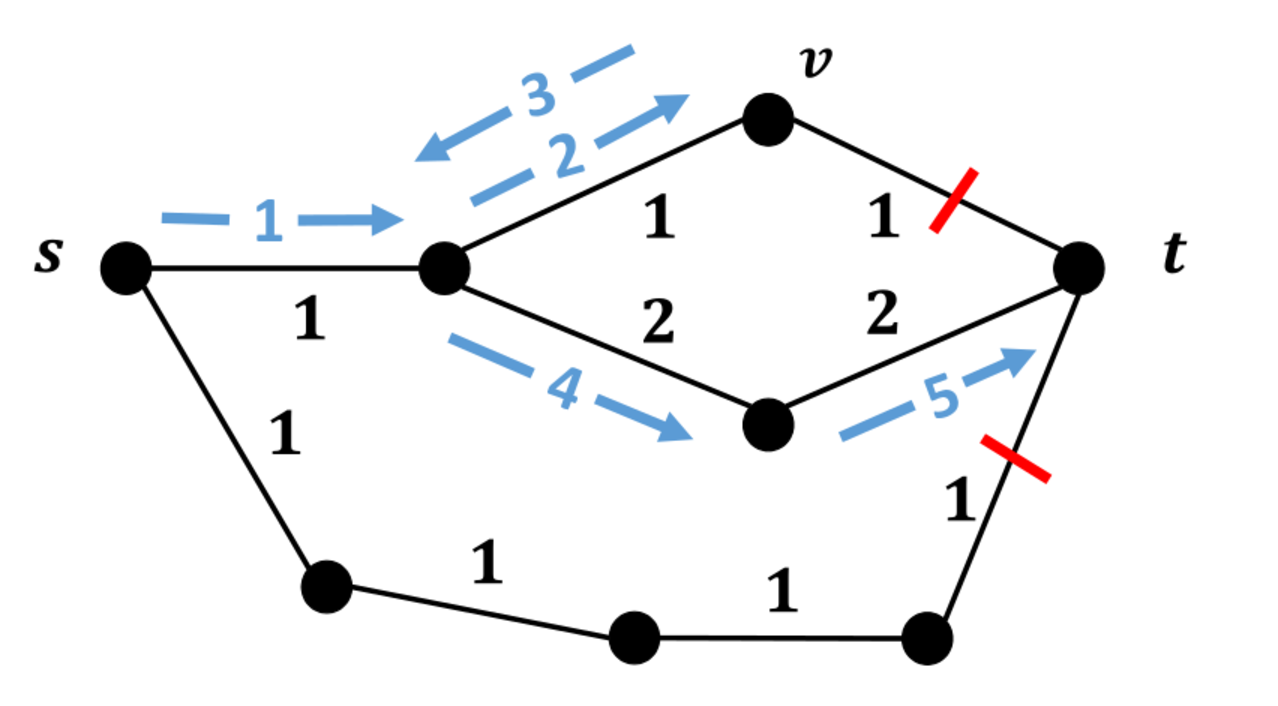
\includegraphics[scale=0.27]{graphics/illustrateCTP2.pdf}
%\caption{Illustration of the \textsc{greedy} strategy on a graph with 2 blocked edges}
%\label{fig:illustrateCTP}
%\end{figure}

We focus on \textit{memoryless strategies} (\mts). Concretely, we suppose that the traveller remembers the blocked edges he has discovered but forgets the nodes which he has already visited. In other words, a decision of an \mts ~is independent of the nodes already visited. In the literature, the term \textit{memoryless} was used in the context of online algorithms (e.g. \textsc{paging problem}~\cite{BoEl98}, \textsc{list update problem}~\cite{Al03}) which take decisions according to the current state, ignoring past events. An \mts ~can be either deterministic or randomized.



\begin{definition}[Memoryless Strategies for the \kctp]
A deterministic \\strategy $A$ is an \mts ~if and only if (iff) the next node $w$ the traveller visits depends on graph $G$ deprived of blocked edges already discovered $E_*'$ and the current traveller position $v$: $w = A\left(G\backslash E_*',v\right)$. Similarly, a randomized strategy $A$ is an \mts ~iff node $w$ is the realization of a discrete random variable $X = A\left(G\backslash E_*',v\right)$.
\end{definition}


%  For the same reason, they do not need any extra memory either.
For example, the \textsc{greedy} strategy~\cite{XuHuSuZh09} is a deterministic \mts . It consists in choosing at each step the first edge of the shortest path between the current node $v$ and the target~$t$. 
%This strategy, illustrated in Figure~\ref{fig:illustrateCTP}, does not refer to anterior moves. 
In contrast, the \textsc{reposition} strategy~\cite{We08} is not an \mts ~as its decision refers to the past moves of the traveller. The polynomial-time strategies proposed in the literature do not use much memory information in the decision-making process. Either they are memoryless or they use a small amount of memory. For example, \textsc{reposition} (deterministic~\cite{We08}, randomized~\cite{BeWe15}) can be implemented with a  one bit memory given that the only information to retain is whether the traveller tries to reach $t$ or returns to $s$.

The following process allows us to identify whether a deterministic strategy $A$ is an \mts . Let us suppose that a traveller $T_1$ follows strategy $A$: he has already visited certain nodes of the graph, he is currently at node $v$ but he has not reached target $t$ yet. Let us imagine a second traveller $T_2$ who is airdropped on node $v$ and is guided by strategy $A$. If the traveller $T_2$ always follows the same path as $T_1$ until reaching $t$, $A$ is a deterministic \mts . If $T_1$ and $T_2$ may follow different paths, then $A$ is not an \mts . Formally, prooving that a strategy is a \mts ~consists in finding the function which transforms the pair $\left(G\backslash E_*,v\right)$ into node $w = A\left(G\backslash E_*',v\right)$.

\subsection{Competitive ratio} \label{subsec:compratio}

Let $\left(G,E_*\right)$ be a \textit{road map}, {\em i.e.} a pair with graph $G=\left(V,E,\omega\right)$ and blocked edges $E_* \subsetneq E$, such that there is an \stpath ~in graph $G\backslash E_*$ (nodes $s$ and $t$ remain in the same connected component when all blocked edges are discovered). We note $\omega_A\left(G,E_*\right)$ the distance traversed by the traveller reaching $t$ with strategy $A$ on graph $G$ with blocked edges $E_*$ and $\omegamin\left(G,E_*\right)$ the cost of the shortest \stpath ~in graph $G\backslash E_*$.

The ratio $\omega_A\left(G,E_*\right)/\omegamin\left(G,E_*\right)$ is abbreviated as $c_A\left(G,E_*\right)$. A strategy $A$ is $c_A$-competitive~\cite{BoEl98,XuHuSuZh09} iff for any $\left(G,E_*\right), \omega_A\left(G,E_*\right) \leq c_A \omegamin\left(G,E_*\right)$. Otherwise stated, for any $\left(G,E_*\right)$, $c_A\left(G,E_*\right) \leq c_A$. If strategy $A$ is randomized, $\omega_A\left(G,E_*\right)$ is replaced by $\mathbb{E}\left(\omega_A\left(G,E_*\right)\right)$ which is the expected distance traversed by the traveller to reach $t$ with strategy $A$. The competitive ratio can also be evaluated on a family $\mathcal{R}$ of road maps, put formally:

\begin{equation}
c_{A,\mathcal{R}} = \max\limits_{\left(G,E_*\right) \in \mathcal{R}} c_A\left(G,E_*\right).
\end{equation}

% See command \cms
This ``local'' competitive ratio fulfils $c_{A,\mathcal{R}} \le c_A$. The definition of the competitive ratio can also be extended to families of strategies. We note $\cms$ the competitive ratio of \mts es, which is the minimum over competitive ratios of any \mts es: $\cms = \min\limits_{A ~\mbox{\scriptsize{\mts}}} c_A$. 
%In the remainder, we identify a set of road maps $\mathcal{R}$ such that the competitive ratio of \mts es on it is $2k+O\left(1\right)$.
\section{Road atlas used to study randomized \mts es} \label{sec:roadatlas}

%We specify \textit{road atlases} $\mathcal{R}_k$, {\em i.e.} sets of road maps, which will be used to evaluate the competitiveness of randomized \mts es. We introduce a family of graphs $G_i$ such that graphs composing these road atlases are subgraphs of $G_i$. 
Before specifying \textit{road atlases} $\mcalr_k$, {\em i.e.} families of road maps we construct to evaluate the competitiveness of randomized \mts es, we need to introduce the concepts used in their definition.

%\subsection{Graphs composing road atlas $\mcalr_k$} \label{subsec:Gi}

We define recursively a sequence of graphs $G_i$ for $i \geq 1$ with weights from $\set{1,\varepsilon}$, $0 < \varepsilon \ll 1$. Graphs $G_1$ and $G_{i+1}$ are represented in Figures~\ref{subfig:G_1} and~\ref{subfig:G_i}, graphs $G_2$ and $G_3$ are shown in Figures~\ref{subfig:G_2} and~\ref{subfig:G_3}. Edges with weight 1 are thicker than edges with weight $\varepsilon$. For any graph $G_i$, axis $\deltavert$ is its vertical axis of symmetry (Figures~\ref{subfig:G_2} and~\ref{subfig:G_3}).

%\begin{figure}[b]
%\centering
%\begin{subfigure}[b]{0.49\columnwidth}
%\centering
%\scalebox{.32}{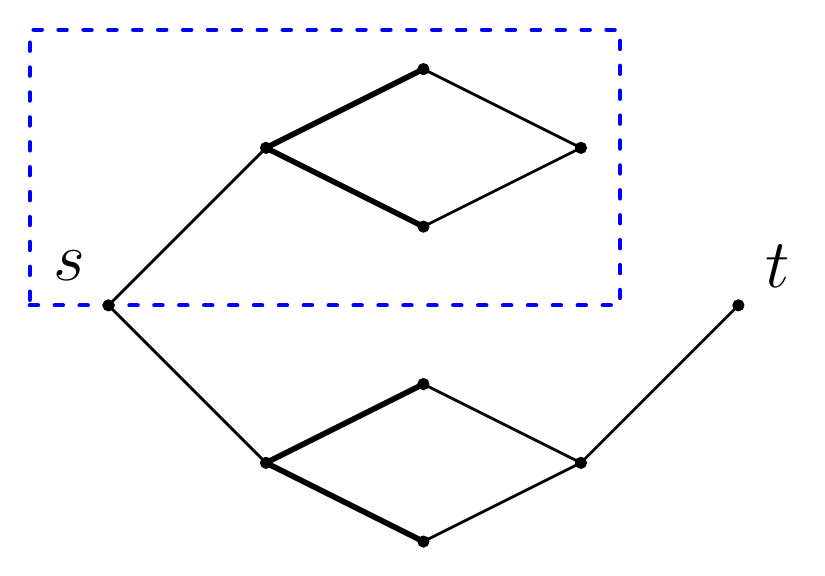
\begin{tikzpicture}[line cap=round,line join=round,>=triangle 45,x=1cm,y=1cm]
%\clip(-7.415949195666677,-4.979207164201812) rectangle (6.110862528225963,7.380468149885891);
\tikzstyle{mydashed}= [dash pattern=on 3pt off 6pt];
\draw [line width=1pt] (0,0)-- (2,2);
\draw [line width=2pt] (2,2)-- (4,3);
\draw [line width=2pt] (2,2)-- (4,1);
\draw [line width=1pt] (4,3)-- (6,2);
\draw [line width=1pt] (4,1)-- (6,2);
%\draw [line width=1pt] (6,2)-- (8,0);
\draw [line width=1pt] (0,0)-- (2,-2);
\draw [line width=2pt] (2,-2)-- (4,-3);
\draw [line width=2pt] (2,-2)-- (4,-1);
\draw [line width=1pt] (4,-3)-- (6,-2);
\draw [line width=1pt] (4,-1)-- (6,-2);
\draw [line width=1pt] (6,-2)-- (8,0);
\begin{scriptsize}
\draw [line width = 1.5pt, color=blue, mydashed] (-1,0)--(6.5,0)--(6.5,3.5)--(-1,3.5)--(-1,0);
%\draw [line width = 1.4pt,color=red] (4,3.5)--(4,-3.5);
%\draw[color=red] (5,3.5) node {\LARGE $\Delta_{\mbox{\large vert}}$};
\draw [fill=black] (2, 2) circle (2pt);
\draw [fill=black] (4, 3) circle (2pt);
\draw [fill=black] (6, 2) circle (2pt);
\draw [fill=black] (4, 1) circle (2pt);
\draw [fill=black] (0, 0) circle (2pt);
\draw [fill=black] (8, 0) circle (2pt);
\draw [fill=black] (2, -2) circle (2pt);
\draw [fill=black] (4, -3) circle (2pt);
\draw [fill=black] (6, -2) circle (2pt);
\draw [fill=black] (4, -1) circle (2pt);
\draw[color=black] (-0.5, 0.5) node {\Huge $s$};
%\draw[color=black] (2.7, 2.8) node {\LARGE \textbf{1}};
%\draw[color=black] (2.7, 1.2) node {\LARGE \textbf{1}};
%\draw[color=black] (2.7, -1.2) node {\LARGE \textbf{1}};
%\draw[color=black] (2.7, -2.8) node {\LARGE \textbf{1}};
\draw[color=black] (8.5, 0.5) node {\Huge $t$};
\end{scriptsize}
\end{tikzpicture}
}
%\caption{Graph $G_2$ deprived of one edge makes appear a dead end (blue dashed box)}
%\label{subfig:deadend_1}
%\end{subfigure}
%\begin{subfigure}[b]{0.49\columnwidth}
%\centering
%\scalebox{.52}{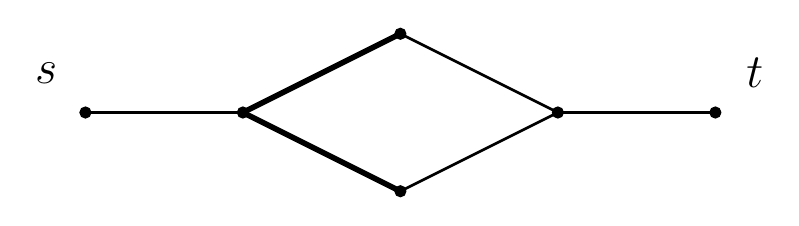
\begin{tikzpicture}[line cap=round,line join=round,>=triangle 45,x=1cm,y=1cm]
%\clip(-7.415949195666677,-4.979207164201812) rectangle (6.110862528225963,7.380468149885891);
%\draw [line width=1pt] (6,2)-- (8,0);
\draw [line width=1pt] (0,0)-- (2,0);
\draw [line width=2pt] (2,0)-- (4,-1);
\draw [line width=2pt] (2,0)-- (4,1);
\draw [line width=1pt] (4,-1)-- (6,0);
\draw [line width=1pt] (4,1)-- (6,0);
\draw [line width=1pt] (6,0)-- (8,0);
\begin{scriptsize}
%\draw [line width = 1.4pt,color=red] (4,3.5)--(4,-3.5);
%\draw[color=red] (5,3.5) node {\LARGE $\Delta_{\mbox{\large vert}}$};
\draw [fill=black] (0, 0) circle (2pt);
\draw [fill=black] (8, 0) circle (2pt);
\draw [fill=black] (2, 0) circle (2pt);
\draw [fill=black] (4, -1) circle (2pt);
\draw [fill=black] (6, 0) circle (2pt);
\draw [fill=black] (4, 1) circle (2pt);
\draw[color=black] (-0.5, 0.5) node {\LARGE $s$};
%\draw[color=black] (2.7, 2.8) node {\LARGE \textbf{1}};
%\draw[color=black] (2.7, 1.2) node {\LARGE \textbf{1}};
%\draw[color=black] (2.7, -1.2) node {\LARGE \textbf{1}};
%\draw[color=black] (2.7, -2.8) node {\LARGE \textbf{1}};
\draw[color=black] (8.5, 0.5) node {\LARGE $t$};
\end{scriptsize}
\end{tikzpicture}
}
%\caption{The graph obtained after deleting all nodes\slash edges forming a dead end}
%\label{subfig:deadend_2}
%\end{subfigure}
%\caption{An illustration of dead ends on graph $G_2$.\mcalg}
%\end{figure}

We focus on a traveller traversing a road map $\left(G_i,E_*\right)$ composed of graph $G_i$ and at most $i$ blocked edges, guided by an \mts . All blocked edges from $E_*$ are on the right side of axis $\deltavert$. Indeed, blocking edges on the left side of $\deltavert$ affects negligibly the total distance traversed by a traveller. Let us suppose that he traverses graph $G_i$ and has already discovered some blocked edges $E' \subseteq E_*$. He now tries to reach $t$ on graph $G_i\backslash E'$, ignoring that the undiscovered blocked edges are $E_*' = E_* \backslash E'$. The graph considered at this step is $G_i\backslash E'$ as past moves are not taken into account. 
%Even if road map $\left(G_i,E_*\right)$ is the instance, an \mts ~might take decisions in function of graphs $G_i\backslash E'$, where $E' \subseteq E_*$.

We note $\mcalg$ the set of all the subgraphs of $G_i$, {\em i.e.} graphs $G_i\backslash E'$ with at most $i$ edges in $E'$ on the right side of $\deltavert$, for any $i \geq 1$. We call them \textit{diamond graphs} because of their appearance, diamonds joined together. Formally, we write $\mcalg = \bigcup_{i=1}^{+\infty} \set{G_i\backslash E' : \card{E'} \leq i}$. For any graph $G \in \mcalg$, we partition its edges, noted $E_G$, into two sets $\eleft{G}$ (on the left side of axis $\deltavert$) and $\eright{G}$ (on the right side of axis $\deltavert$). 
%Road maps $\left(G,E_*\right)$ composing each road atlas $\mcalr_k$ contain graphs $G$ which are in $\mcalg$. 

\begin{figure}[h]
\centering
\begin{subfigure}[b]{0.49\columnwidth}
\centering
\scalebox{.52}{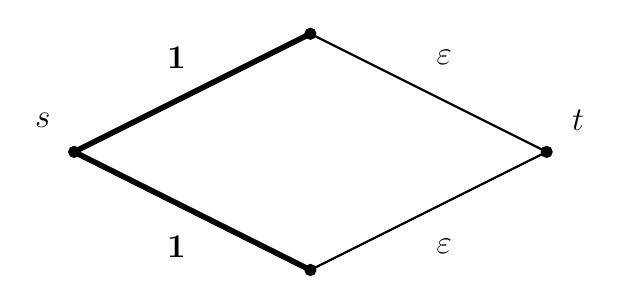
\begin{tikzpicture}[line cap=round,line join=round,>=triangle 45,x=1cm,y=1cm]
%\clip(-6.982493065694897,-13.63448020945784) rectangle (22.448157265896512,6.751180862658525);
\draw [line width=2pt] (0,0)-- (3,1.5);
\draw [line width=0.8pt] (3,1.5)-- (6,0);
\draw [line width=2pt] (0,0)-- (3,-1.5);
\draw [line width=0.8pt] (3,-1.5)-- (6,0);
\begin{scriptsize}\draw [fill=black] (6,0) circle (2pt);
\draw[color=black] (6.4,0.4) node {\large $t$};
\draw [fill=black] (0,0) circle (2pt);
\draw[color=black] (-0.4,0.4) node {\large $s$};
\draw [fill=black] (3,1.5) circle (2pt);
\draw [fill=black] (3,-1.5) circle (2pt);
\draw[color=black] (1.3,1.2) node {\large \bf{1}};
\draw[color=black] (4.7,1.2) node {\large $\varepsilon$};
\draw[color=black] (1.3,-1.2) node {\large \bf{1}};
\draw[color=black] (4.7,-1.2) node {\large $\varepsilon$};
\end{scriptsize}
\end{tikzpicture} }
\caption{Graph $G_1$}
\label{subfig:G_1}
\end{subfigure}
\begin{subfigure}[b]{0.49\columnwidth}
\centering
\scalebox{.52}{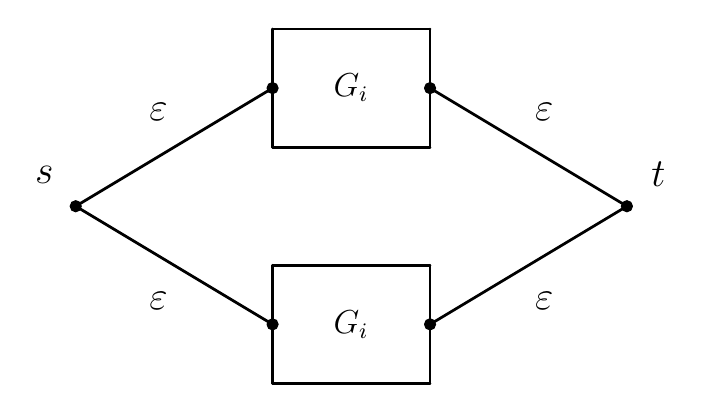
\begin{tikzpicture}[line cap=round,line join=round,>=triangle 45,x=1cm,y=1cm]
\draw [line width=1pt] (0,0)-- (2.5,1.5);
\draw [line width=1pt] (4.5,1.5)-- (7,0);
\draw [line width=1pt] (0,0)-- (2.5,-1.5);
\draw [line width=1pt] (4.5,-1.5)-- (7,0);
\draw [line width=1pt] (2.5,2.25)-- (2.5,0.75);
\draw [line width=1pt] (2.5,0.75)-- (4.5,0.75);
\draw [line width=1pt] (4.5,0.75)-- (4.5,2.25);
\draw [line width=1pt] (4.5,2.25)-- (2.5,2.25);
\draw [line width=1pt] (2.5,-0.75)-- (2.5,-2.25);
\draw [line width=1pt] (2.5,-2.25)-- (4.5,-2.25);
\draw [line width=1pt] (4.5,-2.25)-- (4.5,-0.75);
\draw [line width=1pt] (4.5,-0.75)-- (2.5,-0.75);

\draw (3.15,1.8) node[anchor=north west] {\large $G_i$};
\draw (3.15,-1.2) node[anchor=north west] {\large $G_i$};

\begin{scriptsize}

\draw [fill=black] (0,0) circle (2pt);
\draw[color=black] (-0.4,0.4) node {\Large $s$};
\draw [fill=black] (7,0) circle (2pt);
\draw[color=black] (7.4,0.4) node {\Large $t$};
\draw [fill=black] (2.5,1.5) circle (2pt);
\draw [fill=black] (4.5,1.5) circle (2pt);
\draw [fill=black] (2.5,-1.5) circle (2pt);
\draw [fill=black] (4.5,-1.5) circle (2pt);
\draw[color=black] (1.05,1.2) node {\Large $\varepsilon$};
\draw[color=black] (5.95,1.2) node {\Large $\varepsilon$};
\draw[color=black] (1.05,-1.2) node {\Large $\varepsilon$};
\draw[color=black] (5.95,-1.2) node {\Large $\varepsilon$};

\end{scriptsize}
\end{tikzpicture}}
\caption{Graph $G_{i+1}$}
\label{subfig:G_i}
\end{subfigure}
\begin{subfigure}[b]{0.49\columnwidth}
\centering
\scalebox{.45}{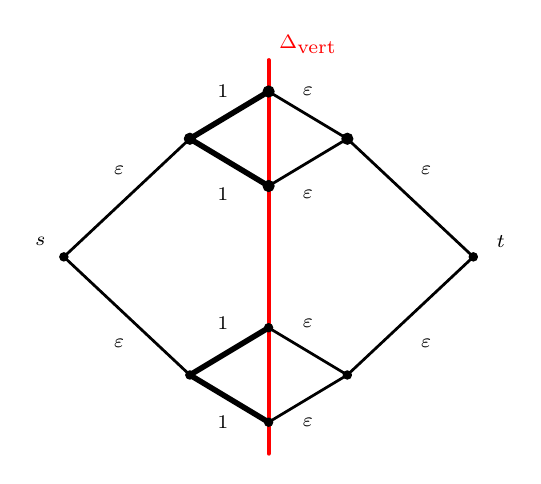
\begin{tikzpicture}[line cap=round,line join=round,>=triangle 45,x=1cm,y=1cm]
%\clip(-7.415949195666677,-4.979207164201812) rectangle (6.110862528225963,7.380468149885891);
\draw [line width=2pt] (-2,4)-- (-1,4.6);
\draw [line width=1pt] (-1,4.6)-- (0,4);
\draw [line width=2pt] (-2,4)-- (-1,3.4);
\draw [line width=1pt] (-1,3.4)-- (0,4);
\draw [line width=1pt] (-3.6,2.5)-- (-2,4);
\draw [line width=1pt] (0,4)-- (1.6,2.5);
\draw [line width=2pt] (-2,1)-- (-1,1.6);
\draw [line width=2pt] (-2,1)-- (-1,0.4);
\draw [line width=1pt] (-1,0.4)-- (0,1);
\draw [line width=1pt] (-1,1.6)-- (0,1);
\draw [line width=1pt] (0,1)-- (1.6,2.5);
\draw [line width=1pt] (-3.6,2.5)-- (-2,1);
\begin{scriptsize}
\draw [line width = 1.4pt,color=red] (-1,0)--(-1,5);
\draw[color=red] (-0.5,5.2) node {$\deltavert$};
\draw [fill=black] (0,4) circle (2pt);
\draw [fill=black] (-2,4) circle (2pt);
\draw [fill=black] (-1,4.6) circle (2pt);
\draw [fill=black] (-1,3.4) circle (2pt);
\draw[color=black] (-1.58,4.6) node {1};
\draw[color=black] (-0.5,4.6) node {$\varepsilon$};
\draw[color=black] (-1.58,3.3) node {1};
\draw[color=black] (-0.5,3.3) node {$\varepsilon$};
\draw [fill=black] (-3.6,2.5) circle (1.5pt);
\draw[color=black] (-3.9,2.7) node {$s$};
\draw[color=black] (-2.9,3.6) node {$\varepsilon$};
\draw [fill=black] (1.6,2.5) circle (1.5pt);
\draw[color=black] (1.95,2.7) node {$t$};
\draw[color=black] (1.0,3.6) node {$\varepsilon$};
\draw [fill=black] (-2,1) circle (1.5pt);
\draw [fill=black] (-1,1.6) circle (1.5pt);
\draw [fill=black] (0,1) circle (1.5pt);
\draw [fill=black] (-1,0.4) circle (1.5pt);
\draw[color=black] (-1.58,1.66) node {1};
\draw[color=black] (-1.58,0.4) node {1};
\draw[color=black] (-0.5,0.4) node {$\varepsilon$};
\draw[color=black] (-0.5,1.66) node {$\varepsilon$};
\draw[color=black] (1.0,1.4) node {$\varepsilon$};
\draw[color=black] (-2.9,1.4) node {$\varepsilon$};
\end{scriptsize}
\end{tikzpicture}
}
\caption{Graph $G_2$ and axis $\deltavert$}
\label{subfig:G_2}
\end{subfigure}
\begin{subfigure}[b]{0.49\columnwidth}
\centering
\scalebox{0.45}{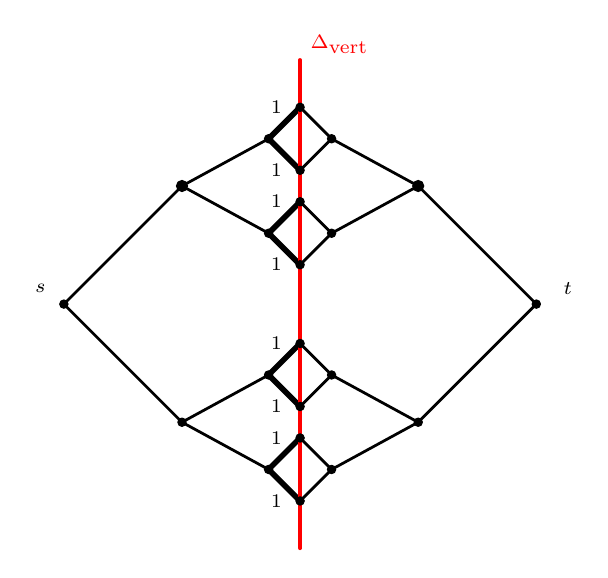
\begin{tikzpicture}[line cap=round,line join=round,>=triangle 45,x=1cm,y=1cm]
%\clip(-7.415949195666677,-5.90693097712365) rectangle (20.34094875546258,7.380468149885891);
\draw [line width=1pt] (-4.0,2.5)-- (-2.5,4);
\draw [line width=1pt] (0.5,4)-- (2.0,2.5);
\draw [line width=1pt] (0.5,1)-- (2.0,2.5);
\draw [line width=1pt] (-4.0,2.5)-- (-2.5,1);
\draw [line width=1pt] (-2.5,4)-- (-1.4,4.6);
\draw [line width=2pt] (-1.4,4.6)-- (-1,5);
\draw [line width=1pt] (-1,5)-- (-0.6,4.6);
\draw [line width=1pt] (-0.6,4.6)-- (-1,4.2);
\draw [line width=2pt] (-1.4,4.6)-- (-1,4.2);
\draw [line width=1pt] (-0.6,4.6)-- (0.5,4);
\draw [line width=1pt] (-2.5,4)-- (-1.4,3.4);
\draw [line width=2pt] (-1.4,3.4)-- (-1,3.8);
\draw [line width=1pt] (-1,3.8)-- (-0.6,3.4);
\draw [line width=2pt] (-1.4,3.4)-- (-1,3);
\draw [line width=1pt] (-1,3)-- (-0.6,3.4);
\draw [line width=1pt] (-0.6,3.4)-- (0.5,4);
\draw [line width=1pt] (-2.5,1)-- (-1.4,1.6);
\draw [line width=2pt] (-1.4,1.6)-- (-1,2);
\draw [line width=2pt] (-1.4,1.6)-- (-1,1.2);
\draw [line width=1pt] (-1,1.2)-- (-0.6,1.6);
\draw [line width=1pt] (-1,2)-- (-0.6,1.6);
\draw [line width=1pt] (-0.6,1.6)-- (0.5,1);
\draw [line width=1pt] (-2.5,1)-- (-1.4,0.4);
\draw [line width=2pt] (-1.4,0.4)-- (-1,0.8);
\draw [line width=1pt] (-1,0.8)-- (-0.6,0.4);
\draw [line width=2pt] (-1.4,0.4)-- (-1,0);
\draw [line width=1pt] (-1,0)-- (-0.6,0.4);
\draw [line width=1pt] (-0.6,0.4)-- (0.5,1);
\begin{scriptsize}
\draw [line width = 1.4pt,color=red] (-1,-0.6)--(-1,5.6);
\draw[color=red] (-0.5,5.8) node {$\deltavert$};
\draw [fill=black] (0.5,4) circle (2pt);
\draw [fill=black] (-2.5,4) circle (2pt);
\draw [fill=black] (-1.4,4.6) circle (1.5pt);
\draw [fill=black] (-1.4,3.4) circle (1.5pt);
\draw [fill=black] (-4.0,2.5) circle (1.5pt);
\draw[color=black] (-4.3,2.7) node {$s$};
\draw [fill=black] (2.0,2.5) circle (1.5pt);
\draw[color=black] (2.4,2.7) node {$t$};
\draw [fill=black] (-2.5,1) circle (1.5pt);
\draw [fill=black] (-1.4,1.6) circle (1.5pt);
\draw [fill=black] (0.5,1) circle (1.5pt);
\draw [fill=black] (-0.6,0.4) circle (1.5pt);
\draw [fill=black] (-0.6,1.6) circle (1.5pt);
\draw [fill=black] (-1.4,0.4) circle (1.5pt);
\draw [fill=black] (-1,2) circle (1.5pt);
\draw [fill=black] (-1,1.2) circle (1.5pt);
\draw [fill=black] (-1,0.8) circle (1.5pt);
\draw [fill=black] (-1,0) circle (1.5pt);
\draw [fill=black] (-0.6,4.6) circle (1.5pt);
\draw [fill=black] (-1,5) circle (1.5pt);
\draw [fill=black] (-1,4.2) circle (1.5pt);
\draw [fill=black] (-1,3.8) circle (1.5pt);
\draw [fill=black] (-1,3) circle (1.5pt);
\draw [fill=black] (-0.6,3.4) circle (1.5pt);
\draw[color=black] (-1.3,5) node {1};
\draw[color=black] (-1.3,4.2) node {1};
\draw[color=black] (-1.3,3.8) node {1};
\draw[color=black] (-1.3,3) node {1};
\draw[color=black] (-1.3,2) node {1};
\draw[color=black] (-1.3,1.2) node {1};
\draw[color=black] (-1.3,0.8) node {1};
\draw[color=black] (-1.3,0) node {1};
\end{scriptsize}
\end{tikzpicture}
}
\caption{Graph $G_3$ and axis $\deltavert$}
\label{subfig:G_3}
\end{subfigure}
\caption{Recursive construction of graphs $G_i$ 
(weights $\varepsilon$ are omitted in Figures~\ref{subfig:G_2} and~\ref{subfig:G_3}).
}
\label{fig:G_i}
\end{figure}

%When the traveller discovers blocked edges in a graph $G \in \mcalg_k$, parts of the graph become \textit{dead ends}. If a traveller visits a dead end, the only chance for him to reach $t$ is to leave it anyway. Dead ends only provide to the traveller additional costs which make the competitive ratio increase. Therefore, the most competitive strategies (memoryless or not) do not visit dead ends. As soon as a dead end appear when the traveller discovers a blockage, we delete it from the graph. Graph $G\backslash E'$ becomes graph $G$ deprived of both edges $E'$ and dead ends. 
%
%We study the competitiveness of \mts es on the road atlas $\mathcal{R}$ composed of road maps with sub-graphs $G_k \backslash E' \in \mcalg_k$ where $\mcalg_k = \set{G_k\backslash E' : \card{E'} \leq k}$ and blocked edges $E_*'$ which fulfil $\card{E'} + \card{E_*'} = k$. Formally,
%\[
%\mathcal{R} = \bigcup\limits_{k=1}^{+\infty} \mathcal{R}_k ~\mbox{with}~ \mathcal{R}_k = \set{\left(G_k\backslash E',E_*'\right): G_k\backslash E' \in \mcalg_k, E' \cap E_*' = \emptyset, \card{E'} + \card{E_*'} = k}
%\]

%\subsection{Diamond binary trees} \label{subsec:dbt}
To any diamond graph $G$ of $\mcalg$, we associate a \textit{diamond binary tree} (\ebt ), noted $T_G$. Tree $T_G$, rooted in $t$, is obtained from the right half of graph $G$ (on the right side of axis $\deltavert$) by successive contractions of edges: any node with a single son is merged with its father (in Figure~\ref{subfig:ebt_2}: edge $\left(t,v_2\right)$ is contracted, $v_2$ merges with $t$). 
%Any node of a \ebt ~is merged with its parent if he has an unique son. 
We note $T_\varnothing$ the empty tree. Any nonempty tree is a triplet $(v, T_a, T_b)$ with a root $v \in V$ and trees $T_a$ and $T_b$. Figures~\ref{subfig:ebt_2} and~\ref{subfig:ebt_3} illustrate the construction of the \ebt . 

\begin{figure}[h]
\centering
%\begin{subfigure}[b]{0.33\columnwidth}
%\centering
%\scalebox{.42}{%\begin{tikzpicture}[line cap=round,line join=round,>=triangle 45,x=1cm,y=1cm]
%%\clip(-7.415949195666677,-5.90693097712365) rectangle (20.34094875546258,7.380468149885891);
%\draw [line width=1pt] (-4.0,2.5)-- (-2.5,4);
%\draw [line width=1pt] (0.5,4)-- (2.0,2.5);
%\draw [line width=1pt] (0.5,1)-- (2.0,2.5);
%\draw [line width=1pt] (-4.0,2.5)-- (-2.5,1);
%\draw [line width=1pt] (-2.5,4)-- (-1.4,4.6);
%\draw [line width=2pt] (-1.4,4.6)-- (-1,5);
%\draw [line width=1pt] (-1,5)-- (-0.6,4.6);
%\draw [line width=1pt] (-0.6,4.6)-- (-1,4.2);
%\draw [line width=2pt] (-1.4,4.6)-- (-1,4.2);
%\draw [line width=1pt] (-0.6,4.6)-- (0.5,4);
%\draw [line width=1pt] (-2.5,4)-- (-1.4,3.4);
%\draw [line width=2pt] (-1.4,3.4)-- (-1,3.8);
%\draw [line width=1pt] (-1,3.8)-- (-0.6,3.4);
%\draw [line width=2pt] (-1.4,3.4)-- (-1,3);
%\draw [line width=1pt] (-1,3)-- (-0.6,3.4);
%\draw [line width=1pt] (-0.6,3.4)-- (0.5,4);
%\draw [line width=1pt] (-2.5,1)-- (-1.4,1.6);
%\draw [line width=2pt] (-1.4,1.6)-- (-1,2);
%\draw [line width=2pt] (-1.4,1.6)-- (-1,1.2);
%\draw [line width=1pt] (-1,1.2)-- (-0.6,1.6);
%\draw [line width=1pt] (-1,2)-- (-0.6,1.6);
%\draw [line width=1pt] (-0.6,1.6)-- (0.5,1);
%\draw [line width=1pt] (-2.5,1)-- (-1.4,0.4);
%\draw [line width=2pt] (-1.4,0.4)-- (-1,0.8);
%\draw [line width=1pt] (-1,0.8)-- (-0.6,0.4);
%\draw [line width=2pt] (-1.4,0.4)-- (-1,0);
%\draw [line width=1pt] (-1,0)-- (-0.6,0.4);
%\draw [line width=1pt] (-0.6,0.4)-- (0.5,1);
%\begin{scriptsize}
%\draw [line width = 1.4pt,color=red] (-1,-0.6)--(-1,5.6);
%\draw[color=red] (-0.5,5.8) node {$\deltavert$};
%\draw [fill=black] (0.5,4) circle (2pt);
%\draw [fill=black] (-2.5,4) circle (2pt);
%\draw [fill=black] (-1.4,4.6) circle (1.5pt);
%\draw [fill=black] (-1.4,3.4) circle (1.5pt);
%\draw [fill=black] (-4.0,2.5) circle (1.5pt);
%\draw[color=black] (-4.3,2.7) node {$s$};
%\draw [fill=black] (2.0,2.5) circle (1.5pt);
%\draw[color=black] (2.4,2.7) node {$t$};
%\draw [fill=black] (-2.5,1) circle (1.5pt);
%\draw [fill=black] (-1.4,1.6) circle (1.5pt);
%\draw [fill=black] (0.5,1) circle (1.5pt);
%\draw [fill=black] (-0.6,0.4) circle (1.5pt);
%\draw [fill=black] (-0.6,1.6) circle (1.5pt);
%\draw [fill=black] (-1.4,0.4) circle (1.5pt);
%\draw [fill=black] (-1,2) circle (1.5pt);
%\draw [fill=black] (-1,1.2) circle (1.5pt);
%\draw [fill=black] (-1,0.8) circle (1.5pt);
%\draw [fill=black] (-1,0) circle (1.5pt);
%\draw [fill=black] (-0.6,4.6) circle (1.5pt);
%\draw [fill=black] (-1,5) circle (1.5pt);
%\draw [fill=black] (-1,4.2) circle (1.5pt);
%\draw [fill=black] (-1,3.8) circle (1.5pt);
%\draw [fill=black] (-1,3) circle (1.5pt);
%\draw [fill=black] (-0.6,3.4) circle (1.5pt);
%\draw[color=black] (-1.3,5) node {1};
%\draw[color=black] (-1.3,4.2) node {1};
%\draw[color=black] (-1.3,3.8) node {1};
%\draw[color=black] (-1.3,3) node {1};
%\draw[color=black] (-1.3,2) node {1};
%\draw[color=black] (-1.3,1.2) node {1};
%\draw[color=black] (-1.3,0.8) node {1};
%\draw[color=black] (-1.3,0) node {1};
%\end{scriptsize}
%\end{tikzpicture}


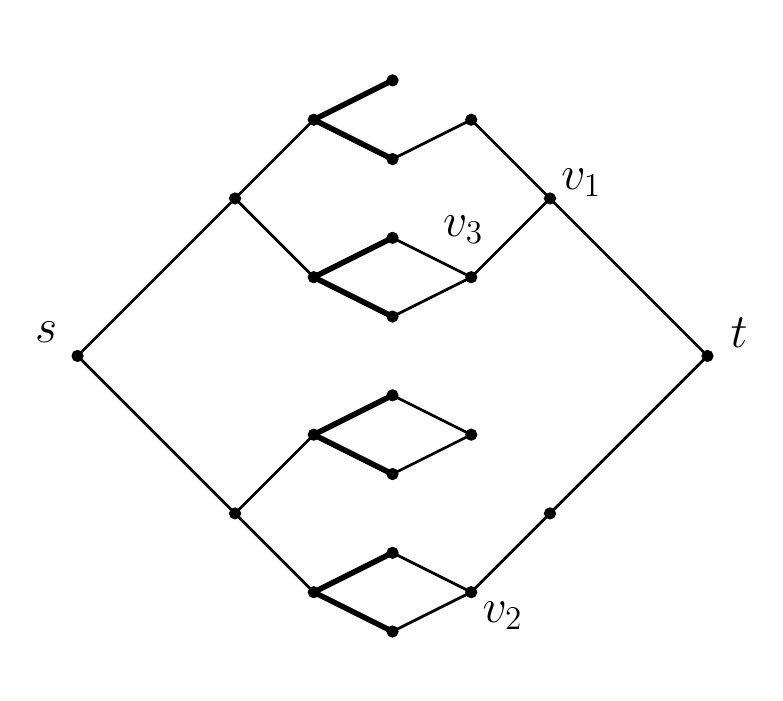
\begin{tikzpicture}[line cap=round,line join=round,>=triangle 45,x=1cm,y=1cm]
%\clip(-7.415949195666677,-4.979207164201812) rectangle (6.110862528225963,7.380468149885891);
\draw [line width=1pt] (-1,0)-- (1,2);
\draw [line width=1pt] (1,2)-- (2,3);
\draw [line width=2pt] (2,3)-- (3,3.5);
\draw [line width=2pt] (2,3)-- (3,2.5);
%\draw [line width=1pt] (3,3.5)-- (4,3);
\draw [line width=1pt] (3,2.5)-- (4,3);
\draw [line width=1pt] (4,3)-- (5,2);
\draw [line width=1pt] (1,2)-- (2,1);
\draw [line width=2pt] (2,1)-- (3,0.5);
\draw [line width=2pt] (2,1)-- (3,1.5);
\draw [line width=1pt] (3,0.5)-- (4,1);
\draw [line width=1pt] (3,1.5)-- (4,1);
\draw [line width=1pt] (4,1)-- (5,2);
\draw [line width=1pt] (5,2)-- (7,0);
\draw [line width=1pt] (-1,0)-- (1,-2);
\draw [line width=1pt] (1,-2)-- (2,-3);
\draw [line width=2pt] (2,-3)-- (3,-3.5);
\draw [line width=2pt] (2,-3)-- (3,-2.5);
\draw [line width=1pt] (3,-3.5)-- (4,-3);
\draw [line width=1pt] (3,-2.5)-- (4,-3);
\draw [line width=1pt] (4,-3)-- (5,-2);
\draw [line width=1pt] (1,-2)-- (2,-1);
\draw [line width=2pt] (2,-1)-- (3,-0.5);
\draw [line width=2pt] (2,-1)-- (3,-1.5);
\draw [line width=1pt] (3,-0.5)-- (4,-1);
\draw [line width=1pt] (3,-1.5)-- (4,-1);
%\draw [line width=1pt] (4,-1)-- (5,-2);
\draw [line width=1pt] (5,-2)-- (7,0);
\begin{scriptsize}
%\draw [line width = 1.4pt,color=red] (3,4)--(3,-4);
%\draw[color=red] (3.8,3.8) node {\LARGE $\Delta_{\mbox{\large vert}}$};
\draw [fill=black] (-1, 0) circle (2pt);
\draw [fill=black] (1, 2) circle (2pt);
\draw [fill=black] (2, 3) circle (2pt);
\draw [fill=black] (3, 3.5) circle (2pt);
\draw [fill=black] (3, 2.5) circle (2pt);
\draw [fill=black] (4, 3) circle (2pt);
\draw [fill=black] (2, 1) circle (2pt);
\draw [fill=black] (3, 1.5) circle (2pt);
\draw [fill=black] (3, 0.5) circle (2pt);
\draw [fill=black] (4, 1) circle (2pt);
\draw [fill=black] (5, 2) circle (2pt);
\draw [fill=black] (1, -2) circle (2pt);
\draw [fill=black] (2, -3) circle (2pt);
\draw [fill=black] (3, -3.5) circle (2pt);
\draw [fill=black] (3, -2.5) circle (2pt);
\draw [fill=black] (4, -3) circle (2pt);
\draw [fill=black] (2, -1) circle (2pt);
\draw [fill=black] (3, -1.5) circle (2pt);
\draw [fill=black] (3, -0.5) circle (2pt);
\draw [fill=black] (4, -1) circle (2pt);
\draw [fill=black] (5, -2) circle (2pt);
\draw [fill=black] (7, 0) circle (2pt);
\draw[color=black] (-1.4, 0.3) node {\LARGE $s$};
\draw[color=black] (5.4, 2.2) node {\LARGE $v_1$};
\draw[color=black] (4.4, -3.3) node {\LARGE $v_2$};
\draw[color=black] (3.9, 1.6) node {\LARGE $v_3$};
%\draw[color=black] (2.6, 3.7) node {\LARGE \textbf{1}};
%\draw[color=black] (2.6, 2.3) node {\LARGE \textbf{1}};
%\draw[color=black] (2.6, 1.7) node {\LARGE \textbf{1}};
%\draw[color=black] (2.6, 0.3) node {\LARGE \textbf{1}};
%\draw[color=black] (2.6, -0.3) node {\LARGE \textbf{1}};
%\draw[color=black] (2.6, -1.7) node {\LARGE \textbf{1}};
%\draw[color=black] (2.6, -2.3) node {\LARGE \textbf{1}};
%\draw[color=black] (2.6, -3.7) node {\LARGE \textbf{1}};
\draw[color=black] (7.4, 0.3) node {\LARGE $t$};
%
\draw[color=white] (3, 4) node {\scriptsize $t$};
\draw[color=white] (3, -3.85) node {\scriptsize $t$};
\end{scriptsize}
\end{tikzpicture}}
%\caption{Graph $G \in \mcalg_3$}
%\label{subfig:ebt_1}
%\end{subfigure}
~
\begin{subfigure}[b]{0.46\columnwidth}
\centering
\scalebox{.42}{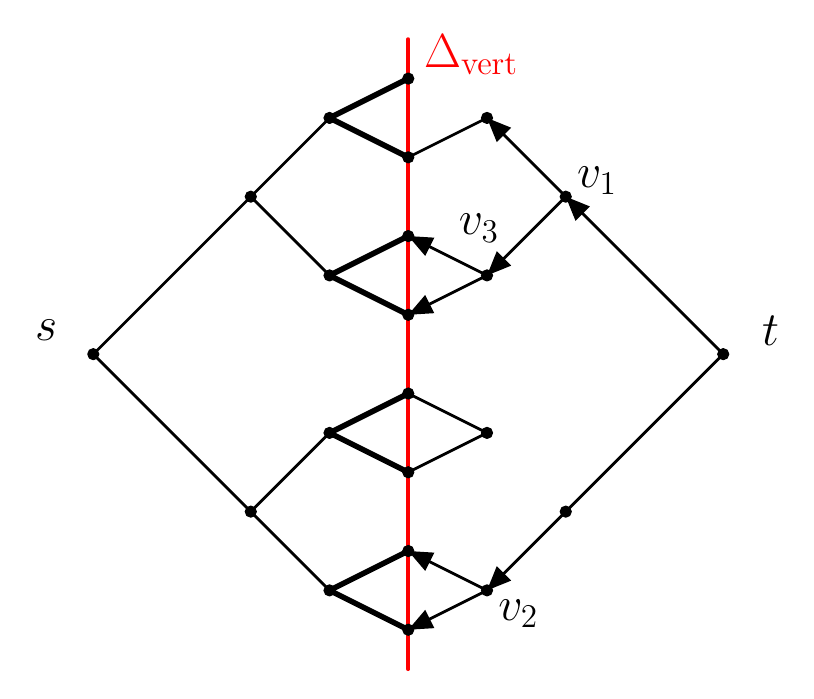
\begin{tikzpicture}[line cap=round,line join=round,>=triangle 45,x=1cm,y=1cm]
%\clip(-7.415949195666677,-4.979207164201812) rectangle (6.110862528225963,7.380468149885891);
\draw [line width=1pt] (-1,0)-- (1,2);
\draw [line width=1pt] (1,2)-- (2,3);
\draw [line width=2pt] (2,3)-- (3,3.5);
\draw [line width=2pt] (2,3)-- (3,2.5);
%\draw [line width=1pt] (3,3.5)-- (4,3);
\draw [line width=1pt,] (3,2.5)-- (4,3);
\draw [line width=1pt,<-] (4,3)-- (5,2);
\draw [line width=1pt] (1,2)-- (2,1);
\draw [line width=2pt] (2,1)-- (3,0.5);
\draw [line width=2pt] (2,1)-- (3,1.5);
\draw [line width=1pt,<-] (3,0.5)-- (4,1);
\draw [line width=1pt,<-] (3,1.5)-- (4,1);
\draw [line width=1pt,<-] (4,1)-- (5,2);
\draw [line width=1pt,<-] (5,2)-- (7,0);
\draw [line width=1pt] (-1,0)-- (1,-2);
\draw [line width=1pt] (1,-2)-- (2,-3);
\draw [line width=2pt] (2,-3)-- (3,-3.5);
\draw [line width=2pt] (2,-3)-- (3,-2.5);
\draw [line width=1pt,<-] (3,-3.5)-- (4,-3);
\draw [line width=1pt,<-] (3,-2.5)-- (4,-3);
\draw [line width=1pt,<-] (4,-3)-- (5,-2);
\draw [line width=1pt] (1,-2)-- (2,-1);
\draw [line width=2pt] (2,-1)-- (3,-0.5);
\draw [line width=2pt] (2,-1)-- (3,-1.5);
\draw [line width=1pt] (3,-0.5)-- (4,-1);
\draw [line width=1pt] (3,-1.5)-- (4,-1);
%\draw [line width=1pt] (4,-1)-- (5,-2);
\draw [line width=1pt] (5,-2)-- (7,0);
\begin{scriptsize}
\draw [line width = 1.4pt,color=red] (3,4)--(3,-4);
\draw[color=red] (3.8,3.8) node {\LARGE $\Delta_{\mbox{\large vert}}$};
\draw [fill=black] (-1, 0) circle (2pt);
\draw [fill=black] (1, 2) circle (2pt);
\draw [fill=black] (2, 3) circle (2pt);
\draw [fill=black] (3, 3.5) circle (2pt);
\draw [fill=black] (3, 2.5) circle (2pt);
\draw [fill=black] (4, 3) circle (2pt);
\draw [fill=black] (2, 1) circle (2pt);
\draw [fill=black] (3, 1.5) circle (2pt);
\draw [fill=black] (3, 0.5) circle (2pt);
\draw [fill=black] (4, 1) circle (2pt);
\draw[color=black] (3.9, 1.6) node {\LARGE $v_3$};
\draw [fill=black] (5, 2) circle (2pt);
\draw[color=black] (5.4, 2.2) node {\LARGE $v_1$};
\draw [fill=black] (1, -2) circle (2pt);
\draw [fill=black] (2, -3) circle (2pt);
\draw [fill=black] (3, -3.5) circle (2pt);
\draw [fill=black] (3, -2.5) circle (2pt);
\draw [fill=black] (4, -3) circle (2pt);
\draw[color=black] (4.4, -3.3) node {\LARGE $v_2$};
\draw [fill=black] (2, -1) circle (2pt);
\draw [fill=black] (3, -1.5) circle (2pt);
\draw [fill=black] (3, -0.5) circle (2pt);
\draw [fill=black] (4, -1) circle (2pt);
\draw [fill=black] (5, -2) circle (2pt);
\draw [fill=black] (7, 0) circle (2pt);
\draw[color=black] (-1.6, 0.3) node {\LARGE $s$};
\draw[color=black] (7.6, 0.3) node {\LARGE $t$};
\end{scriptsize}
\end{tikzpicture}}
\caption{Graph $G \in \mcalg$, subgraph of $G_3$.}
\label{subfig:ebt_2}
\end{subfigure}
~
\begin{subfigure}[b]{0.46\columnwidth}
\centering
\scalebox{.58}{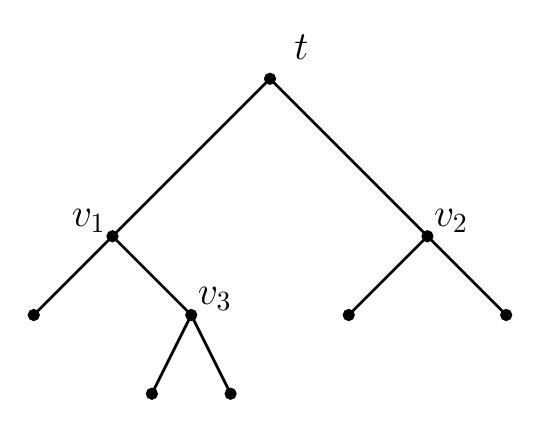
\begin{tikzpicture}[line cap=round,line join=round,>=triangle 45,x=1cm,y=1cm]
%\clip(-7.415949195666677,-4.979207164201812) rectangle (6.110862528225963,7.380468149885891);
\draw [line width=1pt] (3,4)-- (1,2);
\draw [line width=1pt] (3,4)-- (5,2);
\draw [line width=1pt] (1,2)-- (2,1);
\draw [line width=1pt] (1,2)-- (0,1);
\draw [line width=1pt] (2,1)-- (1.5,0);
\draw [line width=1pt] (2,1)-- (2.5,0);
\draw [line width=1pt] (5,2)-- (6,1);
\draw [line width=1pt] (5,2)-- (4,1);
\begin{scriptsize}

%\draw [fill=black] (3, 3.5) circle (2pt);
%\draw [fill=black] (3, 2.5) circle (2pt);
\draw [fill=black] (0, 1) circle (2pt);%fgg
%\draw [fill=black] (2, 1) circle (2pt);
\draw [fill=black] (1.5, 0) circle (2pt);%fgdg
\draw [fill=black] (2.5, 0) circle (2pt);%fgdd
\draw [fill=black] (2, 1) circle (2pt);%fgd 4, 1
\draw[color=black] (2.3, 1.2) node {\Large $v_3$};
\draw [fill=black] (1, 2) circle (2pt);%fg 5,2
\draw[color=black] (0.7, 2.2) node {\Large $v_1$};
%\draw [fill=black] (1, -2) circle (2pt);
%\draw [fill=black] (2, -3) circle (2pt);
\draw [fill=black] (5, 2) circle (2pt);%fd
\draw[color=black] (5.3, 2.2) node {\Large $v_2$};
\draw [fill=black] (6, 1) circle (2pt);%fdd
\draw [fill=black] (4, 1) circle (2pt);%fdg
%\draw [fill=black] (2, -1) circle (2pt);
%\draw [fill=black] (3, -1.5) circle (2pt);
%\draw [fill=black] (3, -0.5) circle (2pt);
%\draw [fill=black] (4, -1) circle (2pt);
%\draw [fill=black] (5, -2) circle (2pt);
\draw [fill=black] (3, 4) circle (2pt);%t 7,0
\draw[color=black] (3.4, 4.4) node {\Large $t$};
\end{scriptsize}
\end{tikzpicture}}
\caption{The \ebt ~$T_G$}
\label{subfig:ebt_3}
\end{subfigure}
\caption{An example of graph $G \in \mcalg$ and its \ebt ~$T_G$.}
\label{fig:ebt}
\end{figure}

To put the definition of \ebt s, let $\dfs\left(v\right)$ denote the set of sons of node $v$. The function $\dfs$ is only defined for the nodes on the right side of $\deltavert$ and for all $v \in \deltavert$, we have $L\left(v\right) = \emptyset$. For graph $G$ of Figure~\ref{subfig:ebt_2}, $\dfs\left(t\right) = \set{v_1,v_2}$, $\dfs\left(v_2\right) = \set{v_4}$, for example. 

Function $\bintree$ gives the construction of tree $T_G$, which is $\bintree \left(t\right)$:
%\command \dfs pour les equations
\[
\bintree\left(v\right) = 
\left\{
\begin{array}{l}
T_\varnothing ~\mbox{if}~ \dfs(v) = \emptyset,\\
\bintree\left(v_{\mbox{\scriptsize{next}}}\right)  ~\mbox{if}~ \dfs(v) = \set{v_{\mbox{\scriptsize{next}}}},\\
\left(v, \bintree(v_{\mbox{\scriptsize{up}}}), \bintree( v_{\mbox{\scriptsize{down}}})\right) ~\mbox{if}~ \dfs(v) = \set{v_{\mbox{\scriptsize{up}}},v_{\mbox{\scriptsize{down}}}}.
\end{array}
\right.
\]
%\begin{algorithm}[]
%\KwData{a directed tree $T$ and a node $v$}
%\KwResult{binary tree}
%\lIf{$deg^-(v) = 0$}{
%	\Return $T_\varnothing$
%}
%\lIf{$deg^-(v) = 1$}{
%	\Return \bintree($T$, $v_{\mbox{\scriptsize{next}}}$)
%}
%\lIf{$deg^-(v) = 2$}{
%	\Return (v, \bintree($T$, $v_{\mbox{\scriptsize{up}}}$), \bintree($T$, $v_{\mbox{\scriptsize{down}}}$)
%}
%\caption{\bintree\ algorithm}
%\label{algo1}
%\end{algorithm}

%Given an edge in a binary tree, we will note $A(e)$ the child edge from above and $B(e)$ the child edge from below. We also note $C(e)$ the set of all the descendants of $e$. Formally, $C(e) = C(A(e)) \cup C(B(e)) \cup \set{A(e), B(e)}$. Finally, we note $P(e)$ the parent edge of $e$ : $P(e) = e' \Leftrightarrow e = A(e') \mbox{ or } e = B(e')$.

%%%%%%%%Commande \dmin pour Dmin
%We introduce notations which characterize nodes of a \ebt . 
We say that the depth of a node $v$ in a \ebt ~$T$, noted $d(v)$, is equal to the number of edges separating it from the root.
%For any edge $e=\left(u,v\right)$ in \ebt ~$T$ where the depth of $u$ is larger than those of $v$, we note $P(e)=\left(v,w\right)$ the ``mother'' edge of $e$ where the depth of $v$ is larger than the depth of $w$. 
We note $\dmin(T)$ the minimum depth of all $T$ leaves. For example, for \ebt ~$T_G$ in Figure~\ref{subfig:ebt_3}, $\dmin(T_G) = 2$. 

\begin{definition}[Sets $\mcald_k$]
Set $\mcald_k$ contains graphs of $\mcalg$ such that their \ebt ~$T_G$ fulfils $\dmin\left(T_G\right) \geq k$: $\mcald_k = \set{G \in \mcalg : \dmin(T_G) \geq k}$. 
\end{definition}

Finally, we define road atlases $\mcalr_k$:

\begin{definition}[Road atlas $\mcalr_k$]
Road atlas $\mcalr_k$ is composed of road maps\\ $\left(G,E_*\right)$, where $\card{E_*} = k$ and $G \in \mcald_k$: $\mcalr_k = \set{\left(G ,E_*\right): G \in \mcald_k \land \card{E_*} = k}$.
\label{def:roadatlas}
\end{definition}
%\[
%\mcalr = \bigcup\limits_{k=1}^{+\infty} \mcalr_k ~\mbox{with}~
%\mcalr_k = \set{\left(G ,E_*\right): G \in \mcald_k, \card{E_*} = k}.
%\]

%Let $U(e)$ denote the ``aunt'' of edge $e$, which has the same parent than $P(e)$. Put formally, $U(e) = \set{e' \in T : P(e') = P\left(P(e)\right) = P^2(e)}$. 
%For any \ebt ~$T$, we define recursively a set of edges $E_T(l)$ which is the set of edges with depth $l$. Set $E_T(0)$ represents the edges connected to the root $t$ and $E_T(l) = \set{e : P(e) \in E_T(l-1)}$. 
%This notation is used in Section~\ref{sec:competitiveness}.

\section{Competitiveness of randomized \mts es} \label{sec:competitiveness}

We study the competitiveness of a randomized \mts ~for road atlases $\mcalr_k$. The \mts ~performance is determined by properties of the corresponding \ebt s $T_G$. These properties result from relations which exist between \ebt ~edges.

The depth of an edge $(u,v)$, $D(u,v)$, is defined as $D(u,v) = \min \set{d(u),d(v)}$. Edge $e'$ is the mother of edge $e$ if $e \cap e' \neq \emptyset$ and $D(e') = D(e) - 1$, putting it shortly $e' = P(e)$. Edge $e^*$ is the aunt of edge $e$ if $e^* \cap P(e) \neq \emptyset$ and $D\left(P(e)\right) = D(e^*)$. We indicate this fact as $e^* = U(e)$. Observe that the aunt of $e$ and its mother share the same ancestor which may be written as $U(e) = \set{e' \in T: P(e') = P(P(e)) = P^2(e)}$.

The following theorem states that cutting one edge from $G \in \mcald_k$ produces a graph $G \backslash \set{e} \in \mcald_{k-1}$.

%%%%%%%%%commande \eright{G} pour dire que l'arete est à droite de deltavert
\begin{theorem}
For any $G \in \mcald_k$ and edge $e \in E_{G, \emph{right}}$, graph $G \backslash \set{e} \in \mcald_{k-1}$.
\label{th:completebinary}
\end{theorem}
\begin{proof}
Let $G \in \mcald_k$ and $e$ be an edge in $\eright{G}$. There is an edge $e^*$ in $T_G$ for which $T_{G \backslash \set{e}}$ is obtained by removing $e^*$ and its descendants from $T_G$ and next applying the edge contraction, if necessary. Let $v$ be the "shallower" endpoint of edge $e^* = \set{u,v}$, {\em i.e.} $d(v) = \min \set{d(u),d(v)}$. Edge $e^*$ and its mother have this node in common, $v \in P\left(e^*\right)$. We distinguish two cases :
%Removing $e$ from $\eright{G}$ makes at least one edge of the \ebt ~$T_G$ disappear and we note $e^*$ the edge among them which is the nearest of $t$ (said differently the edge with lowest depth). Let $v$ be the "root" of edge $e^*$, {\em i.e.} node $v$ such that $e^* = (u, v)$ and $v = P(u)$. We distinguish two cases:
\begin{itemize}[leftmargin=0.3cm]
\item {\bf The depth of node $u$ is greater or equal to $\dmin\left(T_G\right)$:} If $u$ is the unique leaf of depth $\dmin\left(T_G\right)$, the depth of leaves of the \ebt ~$T_{G\backslash \set{e}}$ is $\dmin\left(T_G\right) - 1 \geq k-1$. Otherwise, in \ebt ~$T_{G\backslash \set{e}}$, the depth of leaves is still equal to $\dmin\left(T_G\right) \geq k$. In both cases, $G\backslash \set{e} \in \mcald_{k-1}$.
\item {\bf The depth of node $u$ is strictly inferior to $\dmin\left(T_G\right)$:} Let $T_v$ be the subtree of $T_G$ with root $v$. We note $w$ the brother of node $u$, {\em i.e.} the other son of node $v$ (Figure~\ref{subfig:proofth1_b}). 
%These notations are illustrated in Figure~\ref{subfig:proofth1_a} and~\ref{subfig:proofth1_b}. 
When edge $e$ is removed from $G$, edge $e^*$ and its descendants are withdrawn in the \ebt ~(in the \ebt ~in Figure~\ref{subfig:proofth1_b}, edge $e$ has not been contracted, so $e = e^*$). Consequently, after the contraction, $T_v$ becomes $T_w$, the subtree rooted in~$w$. All the leaves of $T_w$ have initially a depth greater than $k$, so by removing $e$ from $G$, all the leaves of $T_w$ have a depth greater than $k-1$. All leaves outside $T_v$, preserve their depth which is greater than $k$. Therefore, the depth of all leaves of $T_{G \backslash \set{e}}$ is greater than $k-1$.
\end{itemize}
After examining these two cases, we conclude that $G\backslash \set{e}$ belongs to  
$\mcald_{k-1}$.
\end{proof}
%If $E' = \emptyset$, the EBT $T_{G_k}$ is a complete binary tree, so for any $0\le j \le k-1$, $\card{E_{T_{G_k}}(j)}= 2^{j+1}$.
%Let $G_k\backslash E'$ be in $\mcalg_k$ with $\card{E'} = k-D$ and fixed integer $0 < D \le k-1$. As an induction hypothesis, we assume that, for any $G_k\backslash E'' \in \mcalg_k$ with $\card{E''} = k-1-D$, $T_{G_k\backslash E''} \in \compbin{D}$. The objective is to prove that $T_{G_k\backslash E'} \in \compbin{D-1}$ with $D = k-\card{E'}$.
%Then it exists a road map $(G', E_* \cup \set{e})$ with $G$ obtained by removing $e$ to $G'$.
%
% As a consequence, we only need to prove that $\card{E_{T_{G_k\backslash E'}}(j^*-1)} = 2^{j^*}$.
%
%Let $e$ be an arbitrary edge of $E'$. We note $E' = \set{e} \cup E''$ with $\card{E''} = k-D-1$. By hypothesis, graph $G_k\backslash E'' \in \mcalg_k$ fulfils $T_{G_k\backslash E''} \in \compbin{D}$. The EBT $T_{G_k\backslash E''}$ contains edge $e$. We note $v$ the ̀̀̀``root'' of edge $e$, {\em i.e.} node $v$ such that $e = \left(u,v\right)$ and $v = P(u)$. Let $T_v$ be the subtree of $T_{G_k\backslash E''}$ with root $v$ and $w$ be the ``sibling'' of $u$ (said differently the second son of node $v$). When edge $e$ is removed from $G_k\backslash E''$, not only edge $e$ but also its descendants disappear in the EBT and $T_v$ becomes $T_w$, the subtree of root $w$. 
%
%Let $T_{G_k\backslash E''} = \left(t,T_a,T_b\right)$: we assume w.l.o.g. that $e \in T_a$. We know now that $T_{G_k\backslash E'} = \left(t,T_a',T_b\right)$ where $T_a'$ is tree $T_a$ after replacing subtree $T_v$ by $T_w$. As $T_{G_k\backslash E''}$ is complete until depth $D$, $T_a$ and $T_b$ are necessarily complete until edges of depth $D$. When $T_v$ is replaced by $T_w$, the global depth of $T_a$ decreases by 1, so $T_a'$ is complete until depth $D-1$. Eventually, the EBT $T_{G_k\backslash E'} = \left(t,T_a',T_b\right)$ is a binary complete tree from depth 0 to depth $D-1$ (Figures~\ref{subfig:proofth1_b} and~\ref{subfig:proofth1_c}).
%Let $T' = (v, T_a, T_b)$ the sub-tree of $T_G'$ where $v$ is the root of the edge $e$ (we will suppose $e$ is on the $T_a$ side). Then if $e$ is at depth $i$ then the remarks and the hypothesis give $\card{E_{T}(j-i-1)} = 2^{j-i}$ and $\card{E_{T}(j-i-2)} = 2^{j-i-1} = \card{E_{T_a}(j-i-2)}$. By cutting $e$, $T$ become in $G$ the tree $T_a$. We find that the number of edge at the depth $j-i-2$ remains. So the rest of the tree being unchanged by cutting $e$, the number of edges of $T_G$ for depth $j-2$ is unchanged from $T_G'$ and is equal to $2^{j-1}$ : $\card{E_{T_G}(j-2)} = 2^{j-1}$.


\begin{figure}[h]
\centering
\begin{subfigure}[b]{0.3\columnwidth}
\centering
\scalebox{.40}{%\begin{tikzpicture}[line cap=round,line join=round,>=triangle 45,x=1cm,y=1cm]
%%\clip(-7.415949195666677,-5.90693097712365) rectangle (20.34094875546258,7.380468149885891);
%\draw [line width=1pt] (-4.0,2.5)-- (-2.5,4);
%\draw [line width=1pt] (0.5,4)-- (2.0,2.5);
%\draw [line width=1pt] (0.5,1)-- (2.0,2.5);
%\draw [line width=1pt] (-4.0,2.5)-- (-2.5,1);
%\draw [line width=1pt] (-2.5,4)-- (-1.4,4.6);
%\draw [line width=2pt] (-1.4,4.6)-- (-1,5);
%\draw [line width=1pt] (-1,5)-- (-0.6,4.6);
%\draw [line width=1pt] (-0.6,4.6)-- (-1,4.2);
%\draw [line width=2pt] (-1.4,4.6)-- (-1,4.2);
%\draw [line width=1pt] (-0.6,4.6)-- (0.5,4);
%\draw [line width=1pt] (-2.5,4)-- (-1.4,3.4);
%\draw [line width=2pt] (-1.4,3.4)-- (-1,3.8);
%\draw [line width=1pt] (-1,3.8)-- (-0.6,3.4);
%\draw [line width=2pt] (-1.4,3.4)-- (-1,3);
%\draw [line width=1pt] (-1,3)-- (-0.6,3.4);
%\draw [line width=1pt] (-0.6,3.4)-- (0.5,4);
%\draw [line width=1pt] (-2.5,1)-- (-1.4,1.6);
%\draw [line width=2pt] (-1.4,1.6)-- (-1,2);
%\draw [line width=2pt] (-1.4,1.6)-- (-1,1.2);
%\draw [line width=1pt] (-1,1.2)-- (-0.6,1.6);
%\draw [line width=1pt] (-1,2)-- (-0.6,1.6);
%\draw [line width=1pt] (-0.6,1.6)-- (0.5,1);
%\draw [line width=1pt] (-2.5,1)-- (-1.4,0.4);
%\draw [line width=2pt] (-1.4,0.4)-- (-1,0.8);
%\draw [line width=1pt] (-1,0.8)-- (-0.6,0.4);
%\draw [line width=2pt] (-1.4,0.4)-- (-1,0);
%\draw [line width=1pt] (-1,0)-- (-0.6,0.4);
%\draw [line width=1pt] (-0.6,0.4)-- (0.5,1);
%\begin{scriptsize}
%\draw [line width = 1.4pt,color=red] (-1,-0.6)--(-1,5.6);
%\draw[color=red] (-0.5,5.8) node {$\deltavert$};
%\draw [fill=black] (0.5,4) circle (2pt);
%\draw [fill=black] (-2.5,4) circle (2pt);
%\draw [fill=black] (-1.4,4.6) circle (1.5pt);
%\draw [fill=black] (-1.4,3.4) circle (1.5pt);
%\draw [fill=black] (-4.0,2.5) circle (1.5pt);
%\draw[color=black] (-4.3,2.7) node {$s$};
%\draw [fill=black] (2.0,2.5) circle (1.5pt);
%\draw[color=black] (2.4,2.7) node {$t$};
%\draw [fill=black] (-2.5,1) circle (1.5pt);
%\draw [fill=black] (-1.4,1.6) circle (1.5pt);
%\draw [fill=black] (0.5,1) circle (1.5pt);
%\draw [fill=black] (-0.6,0.4) circle (1.5pt);
%\draw [fill=black] (-0.6,1.6) circle (1.5pt);
%\draw [fill=black] (-1.4,0.4) circle (1.5pt);
%\draw [fill=black] (-1,2) circle (1.5pt);
%\draw [fill=black] (-1,1.2) circle (1.5pt);
%\draw [fill=black] (-1,0.8) circle (1.5pt);
%\draw [fill=black] (-1,0) circle (1.5pt);
%\draw [fill=black] (-0.6,4.6) circle (1.5pt);
%\draw [fill=black] (-1,5) circle (1.5pt);
%\draw [fill=black] (-1,4.2) circle (1.5pt);
%\draw [fill=black] (-1,3.8) circle (1.5pt);
%\draw [fill=black] (-1,3) circle (1.5pt);
%\draw [fill=black] (-0.6,3.4) circle (1.5pt);
%\draw[color=black] (-1.3,5) node {1};
%\draw[color=black] (-1.3,4.2) node {1};
%\draw[color=black] (-1.3,3.8) node {1};
%\draw[color=black] (-1.3,3) node {1};
%\draw[color=black] (-1.3,2) node {1};
%\draw[color=black] (-1.3,1.2) node {1};
%\draw[color=black] (-1.3,0.8) node {1};
%\draw[color=black] (-1.3,0) node {1};
%\end{scriptsize}
%\end{tikzpicture}


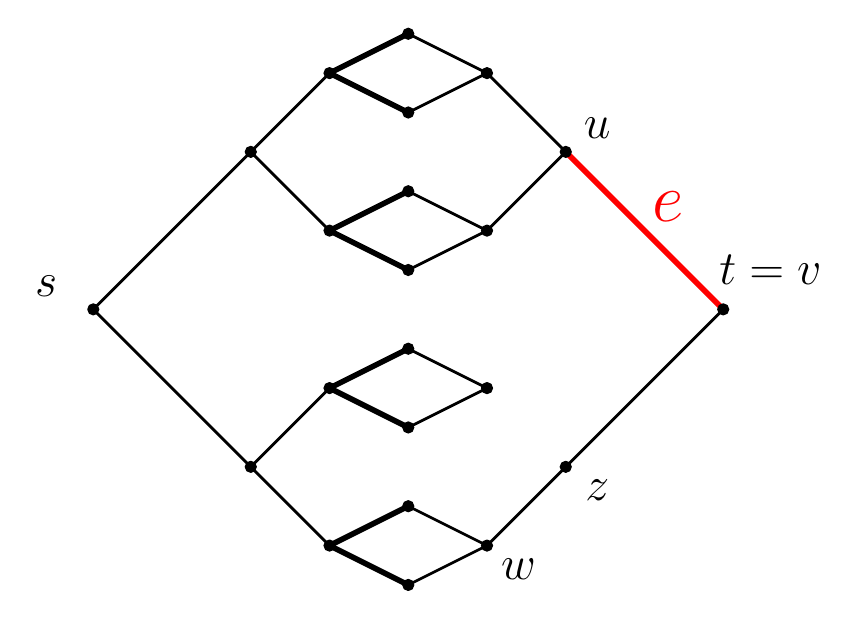
\begin{tikzpicture}[line cap=round,line join=round,>=triangle 45,x=1cm,y=1cm]
%\clip(-7.415949195666677,-4.979207164201812) rectangle (6.110862528225963,7.380468149885891);
\draw [line width=1pt] (-1,0)-- (1,2);
\draw [line width=1pt] (1,2)-- (2,3);
\draw [line width=2pt] (2,3)-- (3,3.5);
\draw [line width=2pt] (2,3)-- (3,2.5);
\draw [line width=1pt] (3,3.5)-- (4,3);
\draw [line width=1pt] (3,2.5)-- (4,3);
\draw [line width=1pt] (4,3)-- (5,2);
\draw [line width=1pt] (1,2)-- (2,1);
\draw [line width=2pt] (2,1)-- (3,0.5);
\draw [line width=2pt] (2,1)-- (3,1.5);
\draw [line width=1pt] (3,0.5)-- (4,1);
\draw [line width=1pt] (3,1.5)-- (4,1);
\draw [line width=1pt] (4,1)-- (5,2);
\draw [line width=2pt,color=red] (5,2)-- (7,0);
\draw[color=red] (6.3, 1.3) node {\Huge $e$};
\draw [line width=1pt] (-1,0)-- (1,-2);
\draw [line width=1pt] (1,-2)-- (2,-3);
\draw [line width=2pt] (2,-3)-- (3,-3.5);
\draw [line width=2pt] (2,-3)-- (3,-2.5);
\draw [line width=1pt] (3,-3.5)-- (4,-3);
\draw [line width=1pt] (3,-2.5)-- (4,-3);
\draw [line width=1pt] (4,-3)-- (5,-2);
\draw [line width=1pt] (1,-2)-- (2,-1);
\draw [line width=2pt] (2,-1)-- (3,-0.5);
\draw [line width=2pt] (2,-1)-- (3,-1.5);
\draw [line width=1pt] (3,-0.5)-- (4,-1);
\draw [line width=1pt] (3,-1.5)-- (4,-1);
%\draw [line width=1pt] (4,-1)-- (5,-2);
\draw [line width=1pt] (5,-2)-- (7,0);
\begin{scriptsize}
%\draw [line width = 1.4pt,color=red] (3,4)--(3,-4);
%\draw[color=red] (3.8,3.8) node {\LARGE $\Delta_{\mbox{\large vert}}$};
\draw [fill=black] (-1, 0) circle (2pt);
\draw [fill=black] (1, 2) circle (2pt);
\draw [fill=black] (2, 3) circle (2pt);
\draw [fill=black] (3, 3.5) circle (2pt);
\draw [fill=black] (3, 2.5) circle (2pt);
\draw [fill=black] (4, 3) circle (2pt);
\draw [fill=black] (2, 1) circle (2pt);
\draw [fill=black] (3, 1.5) circle (2pt);
\draw [fill=black] (3, 0.5) circle (2pt);
\draw [fill=black] (4, 1) circle (2pt);
\draw [fill=black] (5, 2) circle (2pt);
\draw[color=black] (5.4, 2.3) node {\LARGE $u$};
\draw [fill=black] (1, -2) circle (2pt);
\draw [fill=black] (2, -3) circle (2pt);
\draw [fill=black] (3, -3.5) circle (2pt);
\draw [fill=black] (3, -2.5) circle (2pt);
\draw [fill=black] (4, -3) circle (2pt);
\draw[color=black] (4.4, -3.3) node {\LARGE $w$};
\draw [fill=black] (2, -1) circle (2pt);
\draw [fill=black] (3, -1.5) circle (2pt);
\draw [fill=black] (3, -0.5) circle (2pt);
\draw [fill=black] (4, -1) circle (2pt);
\draw [fill=black] (5, -2) circle (2pt);
\draw[color=black] (5.4, -2.3) node {\LARGE $z$};
\draw [fill=black] (7, 0) circle (2pt);
\draw[color=black] (-1.6, 0.3) node {\LARGE $s$};
%\draw[color=black] (5.4, 2.2) node {\LARGE $v_1$};
%\draw[color=black] (4.4, -3.3) node {\LARGE $v_2$};
%\draw[color=black] (3.9, 1.6) node {\LARGE $v_3$};
%\draw[color=black] (2.6, 3.7) node {\LARGE \textbf{1}};
%\draw[color=black] (2.6, 2.3) node {\LARGE \textbf{1}};
%\draw[color=black] (2.6, 1.7) node {\LARGE \textbf{1}};
%\draw[color=black] (2.6, 0.3) node {\LARGE \textbf{1}};
%\draw[color=black] (2.6, -0.3) node {\LARGE \textbf{1}};
%\draw[color=black] (2.6, -1.7) node {\LARGE \textbf{1}};
%\draw[color=black] (2.6, -2.3) node {\LARGE \textbf{1}};
%\draw[color=black] (2.6, -3.7) node {\LARGE \textbf{1}};
\draw[color=black] (7.6, 0.5) node {\LARGE $t=v$};
\end{scriptsize}
\end{tikzpicture}}
\caption{Example of graph $G \in \mcald_2$. Edge $e$ (red) is about to be removed from this graph.}
\label{subfig:proofth1_a}
\end{subfigure}
~
\begin{subfigure}[b]{0.3\columnwidth}
\centering
\scalebox{.55}{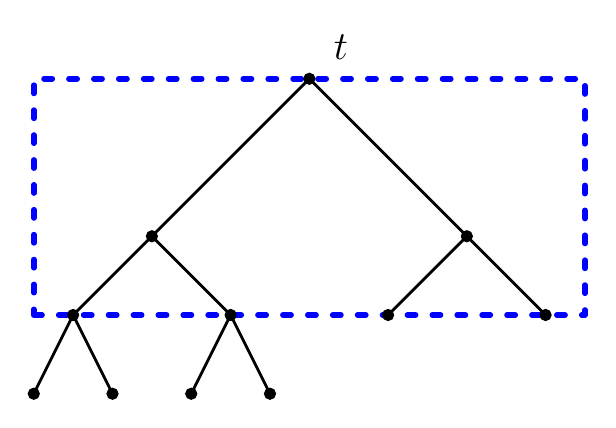
\begin{tikzpicture}[line cap=round,line join=round,>=triangle 45,x=1cm,y=1cm]
%\clip(-7.415949195666677,-4.979207164201812) rectangle (6.110862528225963,7.380468149885891);
\draw [line width=1pt] (3,4)-- (1,2);
\draw [line width=1pt] (3,4)-- (5,2);
\draw [line width=1pt] (1,2)-- (2,1);
\draw [line width=1pt] (1,2)-- (0,1);
\draw [line width=1pt] (2,1)-- (1.5,0);
\draw [line width=1pt] (2,1)-- (2.5,0);
\draw [line width=1pt] (5,2)-- (6,1);
\draw [line width=1pt] (5,2)-- (4,1);
\draw [line width=1pt] (0,1)-- (0.5,0);
\draw [line width=1pt] (0,1)-- (-0.5,0);
\begin{scriptsize}

\tikzstyle{mydashed}= [dash pattern=on 3pt off 6pt];
\draw [line width=2pt, color=blue, mydashed] (-0.5,1)--(6.5,1)--(6.5,4)--(-0.5,4)--(-0.5,1);
%\draw [fill=black] (3, 3.5) circle (2pt);
%\draw [fill=black] (3, 2.5) circle (2pt);
\draw [fill=black] (0, 1) circle (2pt);%fgg
\draw [fill = black] (-0.5,0) circle (2pt);
\draw [fill = black] (0.5,0) circle (2pt);
%\draw [fill=black] (2, 1) circle (2pt);
\draw [fill=black] (1.5, 0) circle (2pt);%fgdg
\draw [fill=black] (2.5, 0) circle (2pt);%fgdd
\draw [fill=black] (2, 1) circle (2pt);%fgd 4, 1
%\draw[color=black] (2.3, 1.2) node {\Large $v_3$};
\draw [fill=black] (1, 2) circle (2pt);%fg 5,2
%\draw[color=black] (0.7, 2.2) node {\Large $v_1$};
%\draw [fill=black] (1, -2) circle (2pt);
%\draw [fill=black] (2, -3) circle (2pt);
\draw [fill=black] (5, 2) circle (2pt);%fd
%\draw[color=black] (5.3, 2.2) node {\Large $v_2$};
\draw [fill=black] (6, 1) circle (2pt);%fdd
\draw [fill=black] (4, 1) circle (2pt);%fdg
%\draw [fill=black] (2, -1) circle (2pt);
%\draw [fill=black] (3, -1.5) circle (2pt);
%\draw [fill=black] (3, -0.5) circle (2pt);
%\draw [fill=black] (4, -1) circle (2pt);
%\draw [fill=black] (5, -2) circle (2pt);
\draw [fill=black] (3, 4) circle (2pt);%t 7,0
\draw[color=black] (3.4, 4.4) node {\Large $t$};
\end{scriptsize}
\end{tikzpicture}}
\caption{The \ebt ~$T_{G}$. Blue frame covers nodes of depth 0 to 2. Two leaves are at depth 2.}
\label{subfig:proofth1_b}
\end{subfigure}
~
\begin{subfigure}[b]{0.3\columnwidth}
\centering
\scalebox{.55}{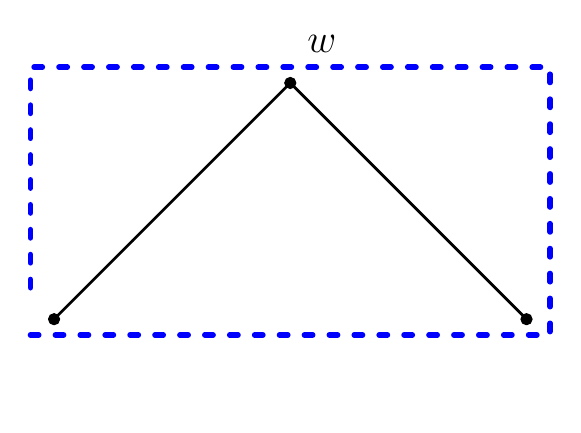
\begin{tikzpicture}[line cap=round,line join=round,>=triangle 45,x=1cm,y=1cm]
%\clip(-7.415949195666677,-4.979207164201812) rectangle (6.110862528225963,7.380468149885891);
\draw [line width=1pt] (3,4)-- (1,2);
\draw [line width=1pt] (3,4)-- (5,2);
%\draw [line width=1pt] (1,2)-- (2,1);
\draw [line width=1pt] (1,2)-- (0,1);
%\draw [line width=1pt] (2,1)-- (1.5,0);
%\draw [line width=1pt] (2,1)-- (2.5,0);
\draw [line width=1pt] (5,2)-- (6,1);
%\draw [line width=1pt] (5,2)-- (4,1);
%\draw [line width=1pt] (0,1)-- (0.5,0);
%\draw [line width=1pt] (0,1)-- (-0.5,0);
\begin{scriptsize}

\tikzstyle{mydashed}= [dash pattern=on 3pt off 6pt];
\draw [line width=2pt, color=blue, mydashed] (-0.3,0.8)--(6.3,0.8)--(6.3,4.2)--(-0.3,4.2)--(-0.3,1.2);
%\draw [fill=black] (3, 3.5) circle (2pt);
%\draw [fill=black] (3, 2.5) circle (2pt);
\draw [fill=black] (0, 1) circle (2pt);%fgg
\draw [fill=white] (0, 0) node {};%fgg
%\draw [fill = black] (-0.5,0) circle (2pt);
%\draw [fill = black] (0.5,0) circle (2pt);
%\draw [fill=black] (2, 1) circle (2pt);
%\draw [fill=black] (1.5, 0) circle (2pt);%fgdg
%\draw [fill=black] (2.5, 0) circle (2pt);%fgdd
%\draw [fill=black] (2, 1) circle (2pt);%fgd 4, 1
%\draw[color=black] (2.3, 1.2) node {\Large $v_3$};
%\draw [fill=black] (1, 2) circle (2pt);%fg 5,2
%\draw[color=black] (0.7, 2.2) node {\Large $v_1$};
%\draw [fill=black] (1, -2) circle (2pt);
%\draw [fill=black] (2, -3) circle (2pt);
%\draw [fill=black] (5, 2) circle (2pt);%fd
%\draw[color=black] (5.3, 2.2) node {\Large $v_2$};
\draw [fill=black] (6, 1) circle (2pt);%fdd
%\draw [fill=black] (4, 1) circle (2pt);%fdg
%\draw [fill=black] (2, -1) circle (2pt);
%\draw [fill=black] (3, -1.5) circle (2pt);
%\draw [fill=black] (3, -0.5) circle (2pt);
%\draw [fill=black] (4, -1) circle (2pt);
%\draw [fill=black] (5, -2) circle (2pt);
\draw [fill=black] (3, 4) circle (2pt);%t 7,0
\draw[color=black] (3.4, 4.5) node {\Large $w$};
\end{scriptsize}
\end{tikzpicture}}
\caption{The \ebt ~$T_{G \backslash \set{e}}$. Nodes of depth 0 to 1 are framed. Graph $G\backslash \set{e}$ belongs to $\mcald_1$.}
\label{subfig:proofth1_c}
\end{subfigure}
\caption{Illustration of the proof of Theorem~\ref{th:completebinary} on a subgraph of $G_3$.}
\label{fig:proofth1}
\end{figure}


We note $\cms\left(G, k\right)$ the maximum over values $\cms\left(G,E_*\right)$, where $\left(G,E_*\right) \in \mcalr_k$. This maximum represents the competitive ratio of \mts es on road maps containing graph $G$ from $\mcald_k$. Formally: 
\begin{equation}
\cms\left(G, k\right) = \min\limits_{A \in ~\mbox{\scriptsize {MS}}} \max\limits_{\left(G,E_*\right) \in \mcalr_k} c_A\left(G,E_*\right).
\label{eq:cmsg}
\end{equation}
Observe that the competitive ratio $\cms(G,k)$ defined for a traveller making the first move from source $s$ is still valid for a traveller starting his walk at any node on the left side of axis $\deltavert$ as weights $\varepsilon$ are negligeable. 

The next theorem states that value $\cms\left(G, k\right)$ is the same for all graphs of $\mcald_k$. In other words, graphs in $\mcald_k$ are equivalent regarding the competitiveness of \mts es. Let $c_k$ denote the competitive ratio of \mts es over atlas $\mcalr_k$. The proof of Theorem~\ref{th:equalcompetitive} provides a recursive formula of ratio $c_k$.

\begin{theorem}
For any graphs $G, G' \in \mcald_k$, $c_{\emph{\scriptsize{MS}}}(G,k) = c_{\emph{\scriptsize{MS}}}(G',k) = c_k$.
\label{th:equalcompetitive}
\end{theorem}
\begin{proof}
We proceed by induction. If $k = 0$, then for every graph of $\mcald_0$, $\cms(G,0) = c_0 = 1$ because any path the traveller takes is open.

We assume that the theorem holds for graphs from $\mcald_{k-1}$. For any $G \in \mcald_k$, all leaves of $T_G$ are at depth greater than or equal to $k$. So, $T_G$ is complete up to depth $k$ and has $2^k$ nodes of depth $k$. We suppose that the traveller, guided by the most competitive \mts ~$A$ over atlas $\mcalr_k$, is standing at source $s$ and starts his walk on a road map $\left(G,E_*\right) \in \mcalr_k$. We determine an upper bound of $c_A(G, E_*)$.

%As strategy $A$ is the most competitive, it makes the traveller traverse exactly a distance 1 (weights $\varepsilon$ are neglected) before reaching $t$ directly or meeting a blocked edge.
%In other words, strategy $A$ does not force the traveller to do superfluous two-way trips. By this way, strategy $A$ is among the most competitive \mts es on road atlas $\mcalr_k$. 
As strategy $A$ is the most competitive, the traveller using it either reaches $t$ directly with distance $1$ or meets a blocked edge and traverses a total distance $2 + c_{k-1}$: distance 1 to reach the blockage, distance 1 to go back to a node on the left hand side of $\deltavert$, and distance $c_{k-1}$ to reach $t$ on graph $G$ deprived of the blocked edges, which belongs to $\mcald_{k-1}$ (Theorem~\ref{th:completebinary}).
%Either the traveller reaches $t$ directly with distance 1 or he meets a blocked edge and traverses a total distance $2 + c_{k-1}$: distance 1 to reach the blockage, distance 1 to go back left to $\deltavert$ and distance $c_{k-1}$ to reach $t$ on graph $G$ deprived of the blocked edges, which belongs to $\mcald_{k-1}$ (see Theorem~\ref{th:completebinary}).

For any $1 \le j \le 2^k$, let $p_{k,j}^A$ signifies the probability that the traveller visits the $\ith{j}$ node at depth $k$, noted $v_{k,j}$ (index $j$ passes from left to right in the \ebt ~representation). 
%Note that $\sum_{j=1}^{2^k} p_{k,j}^A = 1$.
Let $P_{k,j}$ be the set of simple \stpaths ~of length 1 which passes through node $v_{k,j}$.
Given a set $E_*$ of blocked edges, we note $\mcaln(E_*)$ the set of nodes $v_{k,j}$ of depth $k$ such that any path of $P_{k,j}$ is open. For any set of blocked edges, set $\mcaln(E_*)$ is necessarily non-empty because the minimum number of edges needed to block at least one path from each set $P_{k,j}$ is $k+1$. 

For any node $v_{k,j}$, we construct a set of blocked edges such that $\mcaln(E_*) = \set{v_{k,j}}$ and all paths in any $P_{k,j'}$ with $j' \neq j$ are obstructed. Indeed, let $e$ be the edge linking the father node of $v_{k,j}$ and its brother. By blocking the set of edges $E_{k,j}$ containing $e$,  $U(e)$, $U(U(e)),\ldots, U^{k-1}(e)$, we block $1+2+4+\ldots+2^{k-1} = 2^k - 1$ nodes $v_{k,j'}$ at depth $k$, $j' \neq j$. 
%As we consider only simple paths, each path in $P_j$ are open. 
It comes that:
\[
c_A(G, E_{k,j}) = p_{k,j}^A + (2+c_{k-1})\sum_{j' \neq j}p_{k,j'}^A = p_{k,j}^A + (2+c_{k-1})(1-p_{k,j}^A).
\]
For any set of blocked edges $E_*$, if $v_{k,j} \in \mcaln(E_*)$, then the distance traversed when passing through it is $1$. If $v_{k,j} \notin \mcaln(E_*)$, it is at most $2 + c_{k-1}$:
\[
c_A(G, E_*) \leq \sum_{v_{k,j}\in \mcaln(E_*)} p_{k,j}^A+  (2+c_{k-1})\sum_{v_{k,j}\notin \mcaln(E_*)}p_{k,j}^A.
\]

We note $j^*$ the index of the node $v_{k,j^*}$ in $\mcaln\left(E_*\right)$, where $p_{k,j^*}^A$ is the smallest. As $1 < 2 + c_{k-1}$, the greater $\sum_{v_{k,j}\in \mcaln(E_*)} p_{k,j}^A$ is, the smaller $c_A(G, E_*)$ is:
\[
c_A(G, E_*) \le p_{k,j^*}^A + (2+c_{k-1})\sum_{j\neq j^*}p_{k,j}^A = c_A(G, E_{k,j^*}).
\] 

The ratio $c_A(G, E_*)$ attains this upper bound when $E_* = E_{k,j^*}$. Consequently, we obtain the competitive ratio of strategy $A$ over road atlas $\mcalr_k$,
\[
\begin{array}{rl}
c_{A,\mcalr_k} & =  ~\max_{1 \le j \le 2^k} p_{k,j}^{A} + \left(1-p_{k,j}^{A}\right)\left(2+c_{k-1}\right)\\
& \geq ~\cfrac{1}{2^k} + \left(1-\cfrac{1}{2^k}\right)\left(2+c_{k-1}\right).
\end{array}
\]

The \mts ~with the smallest value $c_{A,\mcalr_k}$ fulfils $p_{k,j}^A = \frac{1}{2^k}$ for any $1 \le j \le 2^k$. This value depends on $k$ and $c_{k-1}$, but not on the graph itself. For $G,G' \in \mcald_k$, $\cms(G,k) = \cms(G',k) = c_k = \min_{A} c_{A,\mcalr_k} = \frac{1}{2^k} + \left(1-\frac{1}{2^k}\right)\left(2+c_{k-1}\right)$.
%So for each $E_*$, it exists $E' \in _mcalf$ such that $c_A(G, E_*) \leq c_A(G, E')$. Finally :
%\[
%c_A(G, \mcalr_k) = \max_{j < 2^k} p_j + (1-p_j)(2+c_{k-1}) = p_{min} + (1-p_{min})(2+c_{k-1})
%\]
%with $p_{min}$ the lowest probability. However, $p_{min} \leq \frac{1}{2^k}$ and $c_A(G, \mcalr_k)$ minimum for $p_{min}$ maximum, so $p_{min} = \frac{1}{2^k}$. The result is that $c_{\mts}(G)$ only depend on $k$ and $c_k = \cfrac{1}{2^k} + \left(1-\cfrac{1}{2^k}\right)\left(2+c_{k-1}\right)$
\end{proof}

The Theorem~\ref{th:equalcompetitive} says that, for $k$ blockages, the competitive ratio of \mts es on road atlas $\mcalr_k$ is given by sequence $c_k$. Accordingly, $\cms \le c_k$.
We observe that $c_k - c_{k-1} = 2 - \frac{1}{2^{k}} - \frac{c_{k-1}}{2^{k}}$
and we obtain the following iterative formula:
\[
c_k = 2k+1-\sum_{j=0}^{k-1}\cfrac{c_j+1}{2^{j+1}}.
\]
As $\sum_{j=0}^{+\infty}\cfrac{c_j+1}{2^{j+1}}$ is finite, $c_k = 2k + O(1)$. The numerical computations give $\sum_{j=0}^{10^4}\cfrac{c_j+1}{2^{j+1}} = 3.213$, so the competitive ratio of \mts es is larger than $2k-2.22$. As $c_k$ represents the competitive ratio of the best competitive \mts ~over road atlas $\mcalr_k$, no \mts ~can go below $2k+O\left(1\right)$ in terms of competitiveness.
%%%%%CONCLUSION%%%%%%%
\section{Conclusion and further work} \label{sec:conclusion}

We studied the competitiveness of the \mts es for the \kctp. An \mts ~is a strategy which does not make decisions referring to the anterior moves of the traveller, in other words, the nodes the traveller visited until his current position.

Then, we constructed a series of \kctp ~instances, called road atlases and noted $\mcalr_k$. 
%Identifying an efficient randomized \mts{}es becomes harder when $k$ tends to infinity. 
We foremost concluded that a randomized  \mts ~cannot reach a competitive ratio better than $2k+\mathcal{O}\left(1\right)$ on road atlas $\mcalr_k$. That is to say that we identified an upper bound on the competitive ratio of randomized \mts{}es which is significantly higher than the existing one $k+1$. In future research, if we aim at designing a strategy with competitive ratio $\alpha k + O\left(1\right)$, $\alpha < 2$, we shall focus on strategies which are not only randomized but use memory as well.

\bibliographystyle{plain}
\bibliography{mctp}



\end{document}
